% locking/locking.tex
% mainfile: ../perfbook.tex
% SPDX-License-Identifier: CC-BY-SA-3.0

\QuickQuizChapter{chp:Locking}{Locking}
%
\Epigraph{Locking is the worst general-purpose synchronization mechanism
	  except for all those other mechanisms that
	  have been tried from time to time.}{\emph{With apologies
	  to the memory of Winston Churchill and to whoever he was
	  quoting}}

In recent concurrency research, the role of villain is often played
by locking.
In many papers and presentations,
locking stands accused of promoting deadlocks, convoying, starvation,
unfairness, data races, and all manner of other concurrency sins.
Interestingly enough, the role of workhorse in production-quality
shared-memory parallel software is played by, you guessed it, locking.
This chapter will look into this dichotomy between villain and
hero, as fancifully depicted in
Figures~\ref{fig:locking:Locking: Villain or Slob?}
and~\ref{fig:locking:Locking: Workhorse or Hero?}.

There are a number of reasons behind this Jekyll-and-Hyde dichotomy:

\begin{enumerate}
\item	Many of locking's sins have pragmatic design solutions that
	work well in most cases, for example:
	\begin{enumerate}
	\item	Use of lock hierarchies to avoid deadlock.
	\item	Deadlock-detection tools, for example, the Linux kernel's
		lockdep facility~\cite{JonathanCorbet2006lockdep}.
	\item	Locking-friendly data structures, such as
		arrays, hash tables, and radix trees, which will
		be covered in Chapter~\ref{chp:Data Structures}.
	\end{enumerate}
\item	Some of locking's sins are problems only at high levels of
	contention, levels reached only by poorly designed programs.
\item	Some of locking's sins are avoided by using other synchronization
	mechanisms in concert with locking.
	These other mechanisms include
	statistical counters
	(see Chapter~\ref{chp:Counting}),
	reference counters
	(see Section~\ref{sec:defer:Reference Counting}),
	hazard pointers
	(see Section~\ref{sec:defer:Hazard Pointers}),
	sequence-locking readers
	(see Section~\ref{sec:defer:Sequence Locks}),
	RCU
	(see Section~\ref{sec:defer:Read-Copy Update (RCU)}),
	and simple non-blocking data structures
	(see Section~\ref{sec:advsync:Non-Blocking Synchronization}).
\item	Until quite recently, almost all large shared-memory parallel
	programs were developed in secret, so that it was difficult for
	most researchers to learn of these pragmatic solutions.
\item	Locking works extremely well for some software artifacts
	and extremely poorly for others.
	Developers who have worked on artifacts for which locking
	works well can be expected to have a much more positive
	opinion of locking than those who have worked on artifacts
	for which locking works poorly, as will be discussed in
	Section~\ref{sec:locking:Locking: Hero or Villain?}.
\item	All good stories need a villain, and locking has a long and
	honorable history serving as a research-paper whipping boy.
\end{enumerate}

\QuickQuiz{}
	Just how can serving as a whipping boy be considered to be
	in any way honorable???
\QuickQuizAnswer{
	The reason locking serves as a research-paper whipping boy is
	because it is heavily used in practice.
	In contrast, if no one used or cared about locking, most research
	papers would not bother even mentioning it.
} \QuickQuizEnd

This chapter will give an overview of a number of ways to avoid locking's
more serious sins.

\begin{figure}[tb]
\centering
\resizebox{2in}{!}{\includegraphics{cartoons/r-2014-Locking-the-Slob}}
\caption{Locking: Villain or Slob?}
\ContributedBy{Figure}{fig:locking:Locking: Villain or Slob?}{Melissa Broussard}
\end{figure}

\begin{figure}[tb]
\centering
\resizebox{2in}{!}{\includegraphics{cartoons/r-2014-Locking-the-Hero}}
\caption{Locking: Workhorse or Hero?}
\ContributedBy{Figure}{fig:locking:Locking: Workhorse or Hero?}{Melissa Broussard}
\end{figure}

\section{Staying Alive}
\label{sec:locking:Staying Alive}
%
\epigraph{I work to stay alive.}{\emph{Bette Davis}}

Given that locking stands accused of deadlock and starvation,
one important concern for shared-memory parallel developers is
simply staying alive.
The following sections therefore cover deadlock, livelock, starvation,
unfairness, and inefficiency.

\subsection{Deadlock}
\label{sec:locking:Deadlock}

Deadlock occurs when each of a group of threads is holding at least one
lock while at the same time waiting on a lock held by a member
of that same group.
This happens even in groups containing a single thread when that thread
attempts to acquire a non-recursive lock that it already holds.
Deadlock can therefore occur even given but one thread and one lock!

Without some sort of external intervention, deadlock is forever.
No thread can acquire the lock it is waiting on until that
lock is released by the thread holding it, but the thread holding
it cannot release it until the holding thread acquires the lock that
it is in turn waiting on.

\begin{figure}[tb]
\centering
\resizebox{1.5in}{!}{\includegraphics{locking/DeadlockCycle}}
\caption{Deadlock Cycle}
\label{fig:locking:Deadlock Cycle}
\end{figure}

We can create a directed-graph representation of a deadlock scenario
with nodes for threads and locks, as shown in
Figure~\ref{fig:locking:Deadlock Cycle}.
An arrow from a lock to a thread indicates that the thread holds
the lock, for example, Thread~B holds Locks~2 and~4.
An arrow from a thread to a lock indicates that the thread is waiting
on the lock, for example, Thread~B is waiting on Lock~3.

A deadlock scenario will always contain at least one deadlock cycle.
In Figure~\ref{fig:locking:Deadlock Cycle}, this cycle is
Thread~B, Lock~3, Thread~C, Lock~4, and back to Thread~B.

\QuickQuiz{}
	But the definition of lock-based deadlock only said that each
	thread was holding at least one lock and waiting on another lock
	that was held by some thread.
	How do you know that there is a cycle?
\QuickQuizAnswer{
	Suppose that there is no cycle in the graph.
	We would then have a directed acyclic graph (DAG), which would
	have at least one leaf node.

	If this leaf node was a lock, then we would have a thread
	that was waiting on a lock that wasn't held by any thread,
	counter to the definition.
	In this case the thread would immediately acquire the lock.

	On the other hand, if this leaf node was a thread, then
	we would have a thread that was not waiting on any lock,
	again counter to the definition.
	And in this case, the thread would either be running or
	be blocked on something that is not a lock.
	In the first case, in the absence of infinite-loop bugs,
	the thread will eventually release the lock.
	In the second case, in the absence of a failure-to-wake bug,
	the thread will eventually wake up and release the lock.\footnote{
		Of course, one type of failure-to-wake bug is a
		deadlock that involves not only locks, but also non-lock
		resources.
		But the question really did say ``lock-based deadlock''!}

	Therefore, given this definition of lock-based deadlock, there
	must be a cycle in the corresponding graph.
} \QuickQuizEnd

Although there are some software environments such as database systems
that can recover from an existing deadlock, this approach requires either
that one of the threads be killed or that a lock be forcibly stolen from
one of the threads.
This killing and forcible stealing can be appropriate for transactions,
but is often problematic for kernel and application-level use of locking:
dealing with the resulting partially updated structures can be extremely
complex, hazardous, and error-prone.

Therefore, kernels and applications should instead avoid deadlocks.
Deadlock-avoidance strategies include locking hierarchies
(Section~\ref{sec:locking:Locking Hierarchies}),
local locking hierarchies
(Section~\ref{sec:locking:Local Locking Hierarchies}),
layered locking hierarchies
(Section~\ref{sec:locking:Layered Locking Hierarchies}),
strategies for dealing with APIs containing pointers to locks
(Section~\ref{sec:locking:Locking Hierarchies and Pointers to Locks}),
conditional locking
(Section~\ref{sec:locking:Conditional Locking}),
acquiring all needed locks first
(Section~\ref{sec:locking:Acquire Needed Locks First}),
single-lock-at-a-time designs
(Section~\ref{sec:locking:Single-Lock-at-a-Time Designs}),
and strategies for signal/interrupt handlers
(Section~\ref{sec:locking:Signal/Interrupt Handlers}).
Although there is no deadlock-avoidance strategy that works perfectly
for all situations, there is a good selection of tools to choose from.

\subsubsection{Locking Hierarchies}
\label{sec:locking:Locking Hierarchies}

Locking hierarchies order the locks and prohibit acquiring locks out
of order.
In Figure~\ref{fig:locking:Deadlock Cycle},
we might order the locks numerically, thus forbidding a thread
from acquiring a given lock if it already holds a lock
with the same or a higher number.
Thread~B has violated this hierarchy because it is attempting to
acquire Lock~3 while holding Lock~4.
This violation permitted the deadlock to occur.

Again, to apply a locking hierarchy, order the locks and prohibit
out-of-order lock acquisition.
In large program, it is wise to use tools to enforce your locking
hierarchy~\cite{JonathanCorbet2006lockdep}.

\subsubsection{Local Locking Hierarchies}
\label{sec:locking:Local Locking Hierarchies}

However, the global nature of locking hierarchies make them difficult to
apply to library functions.
After all, the program using a given library function has not even been
written yet, so how can the poor library-function implementor possibly
hope to adhere to the yet-to-be-written program's locking hierarchy?

One special (but common) case is when the library function does not
invoke any of the caller's code.
In this case, the caller's locks will never be acquired while holding
any of the library's locks, so that there cannot be a deadlock cycle
containing locks from both the library and the caller.

\QuickQuiz{}
	Are there any exceptions to this rule, so that there really could be
	a deadlock cycle containing locks from both the library and
	the caller, even given that the library code never invokes
	any of the caller's functions?
\QuickQuizAnswer{
	Indeed there are!
	Here are a few of them:
	\begin{enumerate}
	\item	If one of the library function's arguments is a pointer
		to a lock that this library function acquires, and if
		the library function holds one of its locks while
		acquiring the caller's lock, then we could have a
		deadlock cycle involving both caller and library locks.
	\item	If one of the library functions returns a pointer to
		a lock that is acquired by the caller, and if the
		caller acquires one of its locks while holding the
		library's lock, we could again have a deadlock
		cycle involving both caller and library locks.
	\item	If one of the library functions acquires a lock and
		then returns while still holding it, and if the caller
		acquires one of its locks, we have yet another way
		to create a deadlock cycle involving both caller
		and library locks.
	\item	If the caller has a signal handler that acquires
		locks, then the deadlock cycle can involve both
		caller and library locks.
		In this case, however, the library's locks are
		innocent bystanders in the deadlock cycle.
		That said, please note that acquiring a lock from
		within a signal handler is a no-no in most
		environments---it is not just a bad idea, it
		is unsupported.
		But if you absolutely must acquire a lock in a signal
		handler, be sure to block that signal while holding that
		same lock in thread context.
	\end{enumerate}
} \QuickQuizEnd

But suppose that a library function does invoke the caller's code.
For example, \co{qsort()} invokes a caller-provided comparison function.
A concurrent implementation of \co{qsort()} likely uses locking,
which might result in deadlock in the perhaps-unlikely case where
the comparison function is a
complicated function involving also locking.
How can the library function avoid deadlock?

The golden rule in this case is ``Release all locks before invoking
unknown code.''
To follow this rule, the \co{qsort()} function must release all of its
locks before invoking the comparison function.
Thus \co{qsort()} will not be holding any of its locks while the comparison
function acquires any of the caller's locks, thus avoiding deadlock.

\QuickQuiz{}
	But if \co{qsort()} releases all its locks before invoking
	the comparison function, how can it protect against races
	with other \co{qsort()} threads?
\QuickQuizAnswer{
	By privatizing the data elements being compared
	(as discussed in Chapter~\ref{chp:Data Ownership})
	or through use of deferral mechanisms such as
	reference counting (as discussed in
	Chapter~\ref{chp:Deferred Processing}).
	Or through use of layered locking hierarchies, as described
	in \cref{sec:locking:Layered Locking Hierarchies}.
} \QuickQuizEnd

\begin{figure}[tb]
\centering
\resizebox{3in}{!}{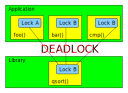
\includegraphics{locking/NonLocalLockHierarchy}}
\caption{Without \tco{qsort()} Local Locking Hierarchy}
\label{fig:locking:Without qsort() Local Locking Hierarchy}
\end{figure}

\begin{figure}[tb]
\centering
\resizebox{3in}{!}{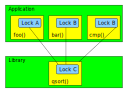
\includegraphics{locking/LocalLockHierarchy}}
\caption{Local Locking Hierarchy for \tco{qsort()}}
\label{fig:locking:Local Locking Hierarchy for qsort()}
\end{figure}

To see the benefits of local locking hierarchies, compare
Figures~\ref{fig:locking:Without qsort() Local Locking Hierarchy} and
\ref{fig:locking:Local Locking Hierarchy for qsort()}.
In both figures, application functions \co{foo()} and \co{bar()}
invoke \co{qsort()} while holding Locks~A and~B, respectively.
Because this is a parallel implementation of \co{qsort()}, it acquires
Lock~C.
Function \co{foo()} passes function \co{cmp()} to \co{qsort()},
and \co{cmp()} acquires Lock~B.
Function \co{bar()} passes a simple integer-comparison function (not
shown) to \co{qsort()}, and this simple function does not acquire any
locks.

Now, if \co{qsort()} holds Lock~C while calling \co{cmp()} in violation
of the golden release-all-locks rule above, as shown in
Figure~\ref{fig:locking:Without qsort() Local Locking Hierarchy},
deadlock can occur.
To see this, suppose that one thread invokes \co{foo()} while a second
thread concurrently invokes \co{bar()}.
The first thread will acquire Lock~A and the second thread will acquire
Lock~B.
If the first thread's call to \co{qsort()} acquires Lock~C, then it
will be unable to acquire Lock~B when it calls \co{cmp()}.
But the first thread holds Lock~C, so the second thread's call to
\co{qsort()} will be unable to acquire it, and thus unable to release
Lock~B, resulting in deadlock.

In contrast, if \co{qsort()} releases Lock~C before invoking the
comparison function, which is unknown code from \co{qsort()}'s perspective,
then deadlock is avoided as shown in
Figure~\ref{fig:locking:Local Locking Hierarchy for qsort()}.

If each module releases all locks before invoking unknown code, then
deadlock is avoided if each module separately avoids deadlock.
This rule therefore greatly simplifies deadlock analysis and greatly
improves modularity.

\subsubsection{Layered Locking Hierarchies}
\label{sec:locking:Layered Locking Hierarchies}

\begin{figure}[tb]
\centering
\resizebox{3in}{!}{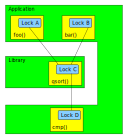
\includegraphics{locking/LayeredLockHierarchy}}
\caption{Layered Locking Hierarchy for \tco{qsort()}}
\label{fig:locking:Layered Locking Hierarchy for qsort()}
\end{figure}

Unfortunately, it might not be possible for \co{qsort()} to release
all of its locks before invoking the comparison function.
In this case, we cannot construct a local locking hierarchy by
releasing all locks before invoking unknown code.
However, we can instead construct a layered locking hierarchy, as shown in
Figure~\ref{fig:locking:Layered Locking Hierarchy for qsort()}.
here, the \co{cmp()} function uses a new Lock~D that is acquired after
all of Locks~A, B, and~C, avoiding deadlock.
We therefore have three layers to the global deadlock hierarchy, the
first containing Locks~A and~B, the second containing Lock~C, and
the third containing Lock~D.

\begin{listing}[tbp]
\input{CodeSamples/locking/locked_list@start_next.fcv}
\caption{Concurrent List Iterator}
\label{lst:locking:Concurrent List Iterator}
\end{listing}

Please note that it is not typically possible to mechanically
change \co{cmp()} to use the new Lock~D.
Quite the opposite: It is often necessary to make profound design-level
modifications.
Nevertheless, the effort required for such modifications is normally
a small price to pay in order to avoid deadlock.
More to the point, this potential deadlock should preferably be detected
at design time, before any code has been generated!

For another example where releasing all locks before invoking unknown
code is impractical, imagine an iterator over a linked list, as shown in
Listing~\ref{lst:locking:Concurrent List Iterator} (\path{locked_list.c}).
The \co{list_start()} function acquires a lock on the list and returns
the first element (if there is one), and
\co{list_next()} either returns a pointer to the next element in the list
or releases the lock and returns \co{NULL} if the end of the list has
been reached.

\begin{listing}[tbp]
\input{CodeSamples/locking/locked_list@list_print.fcv}
\caption{Concurrent List Iterator Usage}
\label{lst:locking:Concurrent List Iterator Usage}
\end{listing}

\begin{fcvref}[ln:locking:locked_list:list_print:ints]
Listing~\ref{lst:locking:Concurrent List Iterator Usage} shows how
this list iterator may be used.
\Clnrefrange{b}{e} define the \co{list_ints} element
containing a single integer,
\end{fcvref}
\begin{fcvref}[ln:locking:locked_list:list_print:print]
and \clnrefrange{b}{e} show how to iterate over the list.
Line~\lnref{start} locks the list and fetches a pointer to the first element,
line~\lnref{entry} provides a pointer to our enclosing \co{list_ints} structure,
line~\lnref{print} prints the corresponding integer, and
line~\lnref{next} moves to the next element.
This is quite simple, and hides all of the locking.
\end{fcvref}

That is, the locking remains hidden as long as the code processing each
list element does not itself acquire a lock that is held across some
other call to \co{list_start()} or \co{list_next()}, which results in
deadlock.
We can avoid the deadlock by layering the locking hierarchy
to take the list-iterator locking into account.

This layered approach can be extended to an arbitrarily large number of layers,
but each added layer increases the complexity of the locking design.
Such increases in complexity are particularly inconvenient for some
types of object-oriented designs, in which control passes back and forth
among a large group of objects in an undisciplined manner.\footnote{
	One name for this is ``object-oriented spaghetti code.''}
This mismatch between the habits of object-oriented design and the
need to avoid deadlock is an important reason why parallel programming
is perceived by some to be so difficult.

Some alternatives to highly layered locking hierarchies are covered in
Chapter~\ref{chp:Deferred Processing}.

\subsubsection{Locking Hierarchies and Pointers to Locks}
\label{sec:locking:Locking Hierarchies and Pointers to Locks}

Although there are some exceptions, an external API containing a pointer
to a lock is very often a misdesigned API.
Handing an internal lock to some other software component is after all
the antithesis of information hiding, which is in turn a key design
principle.

\QuickQuiz{}
	Name one common exception where it is perfectly reasonable
	to pass a pointer to a lock into a function.
\QuickQuizAnswer{
	Locking primitives, of course!
} \QuickQuizEnd

One exception is functions that hand off some entity,
where the caller's lock must be held until the handoff is complete,
but where the lock must be released before the function returns.
One example of such a function is the POSIX \co{pthread_cond_wait()}
function, where passing an pointer to a \co{pthread_mutex_t}
prevents hangs due to lost wakeups.

\QuickQuiz{}
	Doesn't the fact that \co{pthread_cond_wait()} first releases the
	mutex and then re-acquires it eliminate the possibility of deadlock?
\QuickQuizAnswer{
	Absolutely not!

	Consider a program that acquires \co{mutex_a}, and then
	\co{mutex_b}, in that order, and then passes \co{mutex_a}
	to \co{pthread_cond_wait}.
	Now, \co{pthread_cond_wait} will release \co{mutex_a}, but
	will re-acquire it before returning.
	If some other thread acquires \co{mutex_a} in the meantime
	and then blocks on \co{mutex_b}, the program will deadlock.
} \QuickQuizEnd

In short, if you find yourself exporting an API with a pointer to a
lock as an argument or the as the return value, do yourself a favor and
carefully reconsider your API design.
It might well be the right thing to do, but experience indicates that
this is unlikely.

\subsubsection{Conditional Locking}
\label{sec:locking:Conditional Locking}

But suppose that there is no reasonable locking hierarchy.
This can happen in real life, for example, in layered network protocol stacks
where packets flow in both directions.
In the networking case, it might be necessary to hold the locks from
both layers when passing a packet from one layer to another.
Given that packets travel both up and down the protocol stack, this
is an excellent recipe for deadlock, as illustrated in
Listing~\ref{lst:locking:Protocol Layering and Deadlock}.
\begin{fcvref}[ln:locking:Protocol Layering and Deadlock]
Here, a packet moving down the stack towards the wire must acquire
the next layer's lock out of order.
Given that packets moving up the stack away from the wire are acquiring
the locks in order, the lock acquisition in line~\lnref{acq} of the listing
can result in deadlock.
\end{fcvref}

\begin{listing}[tbp]
\begin{fcvlabel}[ln:locking:Protocol Layering and Deadlock]
\begin{VerbatimL}[commandchars=\\\{\}]
spin_lock(&lock2);
layer_2_processing(pkt);
nextlayer = layer_1(pkt);
spin_lock(&nextlayer->lock1);	\lnlbl{acq}
layer_1_processing(pkt);
spin_unlock(&lock2);
spin_unlock(&nextlayer->lock1);
\end{VerbatimL}
\end{fcvlabel}
\caption{Protocol Layering and Deadlock}
\label{lst:locking:Protocol Layering and Deadlock}
\end{listing}

One way to avoid deadlocks in this case is to impose a locking hierarchy,
but when it is necessary to acquire a lock out of order, acquire it
conditionally, as shown in
Listing~\ref{lst:locking:Avoiding Deadlock Via Conditional Locking}.
\begin{fcvref}[ln:locking:Avoiding Deadlock Via Conditional Locking]
Instead of unconditionally acquiring the layer-1 lock, line~\lnref{trylock}
conditionally acquires the lock using the \co{spin_trylock()} primitive.
This primitive acquires the lock immediately if the lock is available
(returning non-zero), and otherwise returns zero without acquiring the lock.

\begin{listing}[tbp]
\begin{fcvlabel}[ln:locking:Avoiding Deadlock Via Conditional Locking]
\begin{VerbatimL}[commandchars=\\\[\]]
retry:
	spin_lock(&lock2);
	layer_2_processing(pkt);
	nextlayer = layer_1(pkt);
	if (!spin_trylock(&nextlayer->lock1)) {	\lnlbl[trylock]
		spin_unlock(&lock2);		\lnlbl[rel2]
		spin_lock(&nextlayer->lock1);	\lnlbl[acq1]
		spin_lock(&lock2);		\lnlbl[acq2]
		if (layer_1(pkt) != nextlayer) {\lnlbl[recheck]
			spin_unlock(&nextlayer->lock1);
			spin_unlock(&lock2);
			goto retry;
		}
	}
	layer_1_processing(pkt);		\lnlbl[l1_proc]
	spin_unlock(&lock2);
	spin_unlock(&nextlayer->lock1);
\end{VerbatimL}
\end{fcvlabel}
\caption{Avoiding Deadlock Via Conditional Locking}
\label{lst:locking:Avoiding Deadlock Via Conditional Locking}
\end{listing}

If \co{spin_trylock()} was successful, line~\lnref{l1_proc} does the needed
layer-1 processing.
Otherwise, line~\lnref{rel2} releases the lock, and
lines~\lnref{acq1} and~\lnref{acq2} acquire them in
the correct order.
Unfortunately, there might be multiple networking devices on
the system (e.g., Ethernet and WiFi), so that the \co{layer_1()}
function must make a routing decision.
This decision might change at any time, especially if the system
is mobile.\footnote{
	And, in contrast to the 1900s, mobility is the common case.}
Therefore, line~\lnref{recheck} must recheck the decision, and if it has changed,
must release the locks and start over.
\end{fcvref}

\QuickQuiz{}
	Can the transformation from
	Listing~\ref{lst:locking:Protocol Layering and Deadlock} to
	Listing~\ref{lst:locking:Avoiding Deadlock Via Conditional Locking}
	be applied universally?
\QuickQuizAnswer{
	Absolutely not!

	This transformation assumes that the
	\co{layer_2_processing()} function is idempotent, given that
	it might be executed multiple times on the same packet when
	the \co{layer_1()} routing decision changes.
	Therefore, in real life, this transformation can become
	arbitrarily complex.
} \QuickQuizEnd

\QuickQuiz{}
	But the complexity in
	Listing~\ref{lst:locking:Avoiding Deadlock Via Conditional Locking}
	is well worthwhile given that it avoids deadlock, right?
\QuickQuizAnswer{
	Maybe.

	If the routing decision in \co{layer_1()} changes often enough,
	the code will always retry, never making forward progress.
	This is termed ``livelock'' if no thread makes any forward progress or
	``starvation''
	if some threads make forward progress but others do not
	(see Section~\ref{sec:locking:Livelock and Starvation}).
} \QuickQuizEnd

\subsubsection{Acquire Needed Locks First}
\label{sec:locking:Acquire Needed Locks First}

In an important special case of conditional locking, all needed
locks are acquired before any processing is carried out.
In this case, processing need not be idempotent: if it turns out
to be impossible to acquire a given lock without first releasing
one that was already acquired, just release all the locks and
try again.
Only once all needed locks are held will any processing be carried out.

However, this procedure can result in \emph{livelock}, which will
be discussed in
Section~\ref{sec:locking:Livelock and Starvation}.

\QuickQuiz{}
	When using the ``acquire needed locks first'' approach described in
	Section~\ref{sec:locking:Acquire Needed Locks First},
	how can livelock be avoided?
\QuickQuizAnswer{
	Provide an additional global lock.
	If a given thread has repeatedly tried and failed to acquire the needed
	locks, then have that thread unconditionally acquire the new
	global lock, and then unconditionally acquire any needed locks.
	(Suggested by Doug Lea.)
} \QuickQuizEnd

A related approach, two-phase locking~\cite{PhilipABernstein1987},
has seen long production use in transactional database systems.
In the first phase of a two-phase locking transaction, locks are
acquired but not released.
Once all needed locks have been acquired, the transaction enters the
second phase, where locks are released, but not acquired.
This locking approach allows databases to provide serializability
guarantees for their transactions, in other words, to guarantee
that all values seen and produced by the transactions are consistent
with some global ordering of all the transactions.
Many such systems rely on the ability to abort transactions, although
this can be simplified by avoiding making any changes to shared data
until all needed locks are acquired.
Livelock and deadlock are issues in such systems, but practical
solutions may be found in any of a number of database textbooks.

\subsubsection{Single-Lock-at-a-Time Designs}
\label{sec:locking:Single-Lock-at-a-Time Designs}

In some cases, it is possible to avoid nesting locks, thus avoiding
deadlock.
For example, if a problem is perfectly partitionable, a single
lock may be assigned to each partition.
Then a thread working on a given partition need only acquire the one
corresponding lock.
Because no thread ever holds more than one lock at a time,
deadlock is impossible.

However, there must be some mechanism to ensure that the needed data
structures remain in existence during the time that neither lock is
held.
One such mechanism is discussed in
Section~\ref{sec:locking:Lock-Based Existence Guarantees}
and several others are presented in
Chapter~\ref{chp:Deferred Processing}.

\subsubsection{Signal/Interrupt Handlers}
\label{sec:locking:Signal/Interrupt Handlers}

Deadlocks involving signal handlers are often quickly dismissed by
noting that it is not legal to invoke \co{pthread_mutex_lock()} from
within a signal handler~\cite{OpenGroup1997pthreads}.
However, it is possible (though often unwise) to hand-craft
locking primitives that \emph{can} be invoked from signal handlers.
Besides which, almost all operating-system kernels permit locks to
be acquired from within interrupt handlers, which are the kernel analog
to signal handlers.

The trick is to block signals (or disable interrupts, as the case may be)
when acquiring any lock that might be acquired within a signal
(or an interrupt) handler.
Furthermore, if holding such a lock, it is illegal to attempt to
acquire any lock that is ever acquired
outside of a signal handler without blocking signals.

\QuickQuiz{}
	Suppose Lock~A is never acquired within a signal handler,
	but Lock~B is acquired both from thread context and by signal
	handlers.
	Suppose further that Lock~A is sometimes acquired with signals
	unblocked.
	Why is it illegal to acquire Lock~A holding Lock~B?
\QuickQuizAnswer{
	Because this would lead to deadlock.
	Given that Lock~A is sometimes held outside of a signal
	handler without blocking signals, a signal might be handled while
	holding this lock.
	The corresponding signal handler might then acquire
	Lock~B, so that Lock~B is acquired while holding Lock~A.
	Therefore, if we also acquire Lock~A while holding Lock~B,
	we will have a deadlock cycle.
	Note that this problem exists even if signals are blocked while
	holding Lock~B.

	This is another reason to be very careful with locks that are
	acquired within interrupt or signal handlers.
	But the Linux kernel's lock dependency checker knows about this
	situation and many others as well, so please do make full use
	of it!
} \QuickQuizEnd

If a lock is acquired by the handlers for several signals, then each
and every one of these signals must be blocked whenever that lock is
acquired, even when that
lock is acquired within a signal handler.

\QuickQuiz{}
	How can you legally block signals within a signal handler?
\QuickQuizAnswer{
	One of the simplest and fastest ways to do so is to use
	the \co{sa_mask} field of the \co{struct sigaction} that
	you pass to \co{sigaction()} when setting up the signal.
} \QuickQuizEnd

Unfortunately, blocking and unblocking signals can be expensive in
some operating systems, notably including Linux, so performance
concerns often mean that locks acquired in signal handlers are only
acquired in signal handlers, and that lockless synchronization
mechanisms are used to communicate between application code and
signal handlers.

Or that signal handlers are avoided completely except for handling
fatal errors.

\QuickQuiz{}
	If acquiring locks in signal handlers is such a bad idea, why
	even discuss ways of making it safe?
\QuickQuizAnswer{
	Because these same rules apply to the interrupt handlers used in
	operating-system kernels and in some embedded applications.

	In many application environments, acquiring locks in signal
	handlers is frowned upon~\cite{OpenGroup1997pthreads}.
	However, that does not stop clever developers from (perhaps
	unwisely) fashioning home-brew locks out of atomic operations.
	And atomic operations are in many cases perfectly legal in
	signal handlers.
} \QuickQuizEnd

\subsubsection{Discussion}
\label{sec:locking:Locking Hierarchy Discussion}

There are a large number of deadlock-avoidance strategies available to
the shared-memory parallel programmer, but there are sequential
programs for which none of them is a good fit.
This is one of the reasons that expert programmers have more than
one tool in their toolbox: locking is a powerful concurrency
tool, but there are jobs better addressed with other tools.

\QuickQuiz{}
	Given an object-oriented application that passes control freely
	among a group of objects such that there is no straightforward
	locking hierarchy,\footnote{
		Also known as ``object-oriented spaghetti code.''}
	layered or otherwise, how can this
	application be parallelized?
\QuickQuizAnswer{
	There are a number of approaches:
	\begin{enumerate}
	\item	In the case of parametric search via simulation,
		where a large number of simulations will be run
		in order to converge on (for example) a good design
		for a mechanical or electrical device, leave the
		simulation single-threaded, but run many instances
		of the simulation in parallel.
		This retains the object-oriented design, and
		gains parallelism at a higher level, and likely
		also avoids synchronization overhead.
	\item	Partition the objects into groups such that there
		is no need to operate on objects in
		more than one group at a given time.
		Then associate a lock with each group.
		This is an example of a single-lock-at-a-time
		design, which discussed in
		Section~\ref{sec:locking:Single-Lock-at-a-Time Designs}.
	\item	Partition the objects into groups such that threads
		can all operate on objects in the groups in some
		groupwise ordering.
		Then associate a lock with each group, and impose a
		locking hierarchy over the groups.
	\item	Impose an arbitrarily selected hierarchy on the locks,
		and then use conditional locking if it is necessary
		to acquire a lock out of order, as was discussed in
		Section~\ref{sec:locking:Conditional Locking}.
	\item	Before carrying out a given group of operations, predict
		which locks will be acquired, and attempt to acquire them
		before actually carrying out any updates.
		If the prediction turns out to be incorrect, drop
		all the locks and retry with an updated prediction
		that includes the benefit of experience.
		This approach was discussed in
		Section~\ref{sec:locking:Acquire Needed Locks First}.
	\item	Use transactional memory.
		This approach has a number of advantages and disadvantages
		which will be discussed in
		Section~\ref{sec:future:Transactional Memory}.
	\item	Refactor the application to be more concurrency-friendly.
		This would likely also have the side effect of making
		the application run faster even when single-threaded, but might
		also make it more difficult to modify the application.
	\item	Use techniques from later chapters in addition to locking.
	\end{enumerate}
} \QuickQuizEnd

Nevertheless, the strategies described in this section have proven
quite useful in many settings.

\subsection{Livelock and Starvation}
\label{sec:locking:Livelock and Starvation}

Although conditional locking can be an effective deadlock-avoidance
mechanism, it can be abused.
Consider for example the beautifully symmetric example shown in
Listing~\ref{lst:locking:Abusing Conditional Locking}.
This example's beauty hides an ugly livelock.
To see this, consider the following sequence of events:

\begin{listing}[tbp]
\begin{fcvlabel}[ln:locking:Abusing Conditional Locking]
\begin{VerbatimL}[commandchars=\\\[\]]
void thread1(void)
{
retry:					\lnlbl[thr1:retry]
	spin_lock(&lock1);		\lnlbl[thr1:acq1]
	do_one_thing();
	if (!spin_trylock(&lock2)) {	\lnlbl[thr1:try2]
		spin_unlock(&lock1);    \lnlbl[thr1:rel1]
		goto retry;
	}
	do_another_thing();
	spin_unlock(&lock2);
	spin_unlock(&lock1);
}

void thread2(void)
{
retry:					\lnlbl[thr2:retry]
	spin_lock(&lock2);		\lnlbl[thr2:acq2]
	do_a_third_thing();
	if (!spin_trylock(&lock1)) {	\lnlbl[thr2:try1]
		spin_unlock(&lock2);	\lnlbl[thr2:rel2]
		goto retry;
	}
	do_a_fourth_thing();
	spin_unlock(&lock1);
	spin_unlock(&lock2);
}
\end{VerbatimL}
\end{fcvlabel}
\caption{Abusing Conditional Locking}
\label{lst:locking:Abusing Conditional Locking}
\end{listing}

\begin{fcvref}[ln:locking:Abusing Conditional Locking]
\begin{enumerate}
\item	Thread~1 acquires \co{lock1} on line~\lnref{thr1:acq1}, then invokes
	\co{do_one_thing()}.
\item	Thread~2 acquires \co{lock2} on line~\lnref{thr2:acq2}, then invokes
	\co{do_a_third_thing()}.
\item	Thread~1 attempts to acquire \co{lock2} on line~\lnref{thr1:try2},
	but fails because Thread~2 holds it.
\item	Thread~2 attempts to acquire \co{lock1} on line~\lnref{thr2:try1},
	but fails because Thread~1 holds it.
\item	Thread~1 releases \co{lock1} on line~\lnref{thr1:rel1},
	then jumps to \co{retry} at line~\lnref{thr1:retry}.
\item	Thread~2 releases \co{lock2} on line~\lnref{thr2:rel2},
	and jumps to \co{retry} at line~\lnref{thr2:retry}.
\item	The livelock dance repeats from the beginning.
\end{enumerate}
\end{fcvref}

\QuickQuiz{}
	How can the livelock shown in
	Listing~\ref{lst:locking:Abusing Conditional Locking}
	be avoided?
\QuickQuizAnswer{
	Listing~\ref{lst:locking:Avoiding Deadlock Via Conditional Locking}
	provides some good hints.
	In many cases, livelocks are a hint that you should revisit your
	locking design.
	Or visit it in the first place if your locking design
	``just grew''.

	That said, one good-and-sufficient approach due to Doug Lea
	is to use conditional locking as described in
	Section~\ref{sec:locking:Conditional Locking}, but combine this
	with acquiring all needed locks first, before modifying shared
	data, as described in
	Section~\ref{sec:locking:Acquire Needed Locks First}.
	If a given critical section retries too many times,
	unconditionally acquire
	a global lock, then unconditionally acquire all the needed locks.
	This avoids both deadlock and livelock, and scales reasonably
	assuming that the global lock need not be acquired too often.
} \QuickQuizEnd

Livelock can be thought of as an extreme form of starvation where
a group of threads starves, rather than just one of them.\footnote{
	Try not to get too hung up on the exact definitions of terms
	like livelock, starvation, and unfairness.
	Anything that causes a group of threads to fail to make adequate
	forward progress is a bug that needs to be fixed, and debating
	names doesn't fix bugs.}

\begin{listing}[tbp]
\begin{fcvlabel}[ln:locking:Conditional Locking and Exponential Backoff]
\begin{VerbatimL}[commandchars=\\\[\]]
void thread1(void)
{
	unsigned int wait = 1;
retry:
	spin_lock(&lock1);
	do_one_thing();
	if (!spin_trylock(&lock2)) {
		spin_unlock(&lock1);
		sleep(wait);
		wait = wait << 1;
		goto retry;
	}
	do_another_thing();
	spin_unlock(&lock2);
	spin_unlock(&lock1);
}

void thread2(void)
{
	unsigned int wait = 1;
retry:
	spin_lock(&lock2);
	do_a_third_thing();
	if (!spin_trylock(&lock1)) {
		spin_unlock(&lock2);
		sleep(wait);
		wait = wait << 1;
		goto retry;
	}
	do_a_fourth_thing();
	spin_unlock(&lock1);
	spin_unlock(&lock2);
}
\end{VerbatimL}
\end{fcvlabel}
\caption{Conditional Locking and Exponential Backoff}
\label{lst:locking:Conditional Locking and Exponential Backoff}
\end{listing}

Livelock and starvation are serious issues in software transactional
memory implementations, and so the concept of \emph{contention
manager} has been introduced to encapsulate these issues.
In the case of locking, simple exponential backoff can often address
livelock and starvation.
The idea is to introduce exponentially increasing delays before each
retry, as shown in
Listing~\ref{lst:locking:Conditional Locking and Exponential Backoff}.

\QuickQuiz{}
	What problems can you spot in the code in
	Listing~\ref{lst:locking:Conditional Locking and Exponential Backoff}?
\QuickQuizAnswer{
	Here are a couple:
	\begin{enumerate}
	\item	A one-second wait is way too long for most uses.
		Wait intervals should begin with roughly the time
		required to execute the critical section, which will
		normally be in the microsecond or millisecond range.
	\item	The code does not check for overflow.
		On the other hand, this bug is nullified
		by the previous bug: 32 bits worth of seconds is
		more than 50 years.
	\end{enumerate}
} \QuickQuizEnd

For better results, backoffs should be bounded, and
even better high-contention results are obtained via queued
locking~\cite{Anderson90}, which is discussed more in
Section~\ref{sec:locking:Other Exclusive-Locking Implementations}.
Of course, best of all is to use a good parallel design that avoids
these problems by maintaining low lock contention.

\subsection{Unfairness}
\label{sec:locking:Unfairness}

\begin{figure}[tb]
\centering
\resizebox{3in}{!}{\includegraphics{cpu/SystemArch}}
\caption{System Architecture and Lock Unfairness}
\label{fig:locking:System Architecture and Lock Unfairness}
\end{figure}

Unfairness can be thought of as a less-severe form of starvation,
where a subset of threads contending for a given lock are granted
the lion's share of the acquisitions.
This can happen on machines with shared caches or NUMA characteristics,
for example, as shown in
Figure~\ref{fig:locking:System Architecture and Lock Unfairness}.
If CPU~0 releases a lock that all the other CPUs are attempting
to acquire, the interconnect shared between CPUs~0 and~1 means that
CPU~1 will have an advantage over CPUs~2--7.
Therefore CPU~1 will likely acquire the lock.
If CPU~1 holds the lock long enough for CPU~0 to be requesting the
lock by the time CPU~1 releases it and vice versa, the lock can
shuttle between CPUs~0 and~1, bypassing CPUs~2--7.
\noclub[1]

\QuickQuiz{}
	Wouldn't it be better just to use a good parallel design
	so that lock contention was low enough to avoid unfairness?
\QuickQuizAnswer{
	It would be better in some sense, but there are situations
	where it can be appropriate to use
	designs that sometimes result in high lock contentions.

	For example, imagine a system that is subject to a rare error
	condition.
	It might well be best to have a simple error-handling design
	that has poor performance and scalability for the duration of
	the rare error condition, as opposed to a complex and
	difficult-to-debug design that is helpful only when one of
	those rare error conditions is in effect.

	That said, it is usually worth putting some effort into
	attempting to produce a design that both simple as well as
	efficient during error conditions, for example by partitioning
	the problem.
} \QuickQuizEnd

\subsection{Inefficiency}
\label{sec:locking:Inefficiency}

Locks are implemented using atomic instructions and memory barriers,
and often involve cache misses.
As we saw in Chapter~\ref{chp:Hardware and its Habits},
these instructions are quite expensive, roughly two
orders of magnitude greater overhead than simple instructions.
This can be a serious problem for locking: If you protect a single
instruction with a lock, you will increase the overhead by a factor
of one hundred.
Even assuming perfect scalability, \emph{one hundred} CPUs would
be required to keep up with a single CPU executing the same code
without locking.

This situation underscores the synchronization\-/granularity
tradeoff discussed in Section~\ref{sec:SMPdesign:Synchronization Granularity},
especially Figure~\ref{fig:SMPdesign:Synchronization Efficiency}:
Too coarse a granularity will limit scalability, while too fine a
granularity will result in excessive synchronization overhead.

That said, once a lock is held, the data protected by that lock can
be accessed by the lock holder without interference.
Acquiring a lock might be expensive, but once held, the CPU's caches
are an effective performance booster, at least for large critical sections.

\QuickQuiz{}
	How might the lock holder be interfered with?
\QuickQuizAnswer{
	If the data protected by the lock is in the same cache line
	as the lock itself, then attempts by other CPUs to acquire
	the lock will result in expensive cache misses on the part
	of the CPU holding the lock.
	This is a special case of false sharing, which can also occur
	if a pair of variables protected by different locks happen
	to share a cache line.
	In contrast, if the lock is in a different cache line than
	the data that it protects, the CPU holding the lock will
	usually suffer a cache miss only on first access to a given
	variable.

	Of course, the downside of placing the lock and data into separate
	cache lines is that the code will incur two cache misses rather
	than only one in the uncontended case.
	As always, choose wisely!
} \QuickQuizEnd

\section{Types of Locks}
\label{sec:locking:Types of Locks}
%
\epigraph{Only locks in life are what you think you know, but don't.
	  Accept your ignorance and try something new.}
	 {\emph{Dennis Vickers}}

There are a surprising number of types of locks, more than this
short chapter can possibly do justice to.
The following sections discuss
exclusive locks (Section~\ref{sec:locking:Exclusive Locks}),
reader-writer locks (Section~\ref{sec:locking:Reader-Writer Locks}),
multi-role locks (Section~\ref{sec:locking:Beyond Reader-Writer Locks}),
and scoped locking (Section~\ref{sec:locking:Scoped Locking}).

\subsection{Exclusive Locks}
\label{sec:locking:Exclusive Locks}

Exclusive locks are what they say they are: only one thread may hold
the lock at a time.
The holder of such a lock thus has exclusive access to all data protected
by that lock, hence the name.

Of course, this all assumes that this lock is held across all accesses
to data purportedly protected by the lock.
Although there are some tools that can help (see for example
Section~\ref{sec:formal:Axiomatic Approaches and Locking}),
the ultimate responsibility for ensuring that the lock is acquired in
all necessary code paths rests with the developer.

\QuickQuiz{}
	Does it ever make sense to have an exclusive lock acquisition
	immediately followed by a release of that same lock, that is,
	an empty critical section?
\QuickQuizAnswer{
	This usage is rare, but is occasionally used.
	The point is that the semantics of exclusive locks have two
	components: (1)~the familiar data-protection semantic and
	(2)~a messaging semantic, where releasing a given lock notifies
	a waiting acquisition of that same lock.
	An empty critical section uses the messaging component without
	the data-protection component.

	The rest of this answer provides some example uses of empty
	critical sections, however, these examples should be considered
	``gray magic.''\footnote{
		Thanks to Alexey Roytman for this description.}
	As such, empty critical sections are almost never used in practice.
	Nevertheless, pressing on into this gray area \ldots

	One historical use of empty critical sections appeared in the
	networking stack of the 2.4 Linux kernel.
	This usage pattern can be thought of as a way of approximating
	the effects of read-copy update (RCU), which is discussed in
	Section~\ref{sec:defer:Read-Copy Update (RCU)}.

	The empty-lock-critical-section idiom can also be used to
	reduce lock contention in some situations.
	For example, consider a multithreaded user-space application where
	each thread processes units of work maintained in a per-thread
	list, where threads are prohibited from touching each others'
	lists.
	There could also be updates that require that all previously
	scheduled units of work have completed before the update can
	progress.
	One way to handle this is to schedule a unit of work on each
	thread, so that when all of these units of work complete, the
	update may proceed.

	In some applications, threads can come and go.
	For example, each thread might correspond to one user of the
	application, and thus be removed when that user logs out or
	otherwise disconnects.
	In many applications, threads cannot depart atomically: They must
	instead explicitly unravel themselves from various portions of
	the application using a specific sequence of actions.
	One specific action will be refusing to accept further requests
	from other threads, and another specific action will be disposing
	of any remaining units of work on its list, for example, by
	placing these units of work in a global work-item-disposal list
	to be taken by one of the remaining threads.
	(Why not just drain the thread's work-item list by executing
	each item?
	Because a given work item might generate more work items, so
	that the list could not be drained in a timely fashion.)

	If the application is to perform and scale well, a good locking
	design is required.
	One common solution is to have a global lock (call it \co{G})
	protecting the entire
	process of departing (and perhaps other things as well),
	with finer-grained locks protecting the
	individual unraveling operations.

	Now, a departing thread must clearly refuse to accept further
	requests before disposing of the work on its list, because
	otherwise additional work might arrive after the disposal action,
	which would render that disposal action ineffective.
	So simplified pseudocode for a departing thread might be as follows:

	\begin{enumerate}
	\item	Acquire lock \co{G}.
	\item	Acquire the lock guarding communications.
	\item	Refuse further communications from other threads.
	\item	Release the lock guarding communications.
	\item	Acquire the lock guarding the global work-item-disposal list.
	\item	Move all pending work items to the global
		work-item-disposal list.
	\item	Release the lock guarding the global work-item-disposal list.
	\item	Release lock \co{G}.
	\end{enumerate}

	Of course, a thread that needs to wait for all pre-existing work
	items will need to take departing threads into account.
	To see this, suppose that this thread starts waiting for all
	pre-existing work items just after a departing thread has refused
	further communications from other threads.
	How can this thread wait for the departing thread's work items
	to complete, keeping in mind that threads are not allowed to
	access each others' lists of work items?

	One straightforward approach is for this thread to acquire \co{G}
	and then the lock guarding the global work-item-disposal list, then
	move the work items to its own list.
	The thread then release both locks,
	places a work item on the end of its own list,
	and then wait for all of the work items that it placed on each thread's
	list (including its own) to complete.

	This approach does work well in many cases, but if special
	processing is required for each work item as it is pulled in
	from the global work-item-disposal list, the result could be
	excessive contention on \co{G}.
	One way to avoid that contention is to acquire \co{G} and then
	immediately release it.
	Then the process of waiting for all prior work items look
	something like the following:

	\begin{enumerate}
	\item	Set a global counter to one and initialize a condition
		variable to zero.
	\item	Send a message to all threads to cause them to atomically
		increment the global counter, and then to enqueue a
		work item.
		The work item will atomically decrement the global
		counter, and if the result is zero, it will set a
		condition variable to one.
	\item	Acquire \co{G}, which will wait on any currently departing
		thread to finish departing.
		Because only one thread may depart at a time, all the
		remaining threads will have already received the message
		sent in the preceding step.
	\item	Release \co{G}.
	\item	Acquire the lock guarding the global work-item-disposal list.
	\item	Move all work items from the global work-item-disposal list
		to this thread's list, processing them as needed along the way.
	\item	Release the lock guarding the global work-item-disposal list.
	\item	Enqueue an additional work item onto this thread's list.
		(As before, this work item will atomically decrement
		the global counter, and if the result is zero, it will
		set a condition variable to one.)
	\item	Wait for the condition variable to take on the value one.
	\end{enumerate}

	Once this procedure completes, all pre-existing work items are
	guaranteed to have completed.
	The empty critical sections are using locking for messaging as
	well as for protection of data.
} \QuickQuizEnd

\QuickQuizLabel{\QlockingQemptycriticalsection}

It is important to note that unconditionally acquiring an exclusive lock
has two effects:
(1)~Waiting for all prior holders of that lock to release it, and
(2)~Blocking any other acquisition attempts until the lock is released.
As a result, at lock acquisition time, any concurrent acquisitions of
that lock must be partitioned into prior holders and subsequent
holders.
Different types of exclusive locks use different partitioning
strategies~\cite{BjoernBrandenburgPhD,Guerraoui:2019:LPA:3319851.3301501},
for example:

\begin{enumerate}
\item	Strict FIFO, with acquisitions starting earlier acquiring
	the lock earlier.
\item	Approximate FIFO, with acquisitions starting sufficiently
	earlier acquiring the lock earlier.
\item	FIFO within priority level, with higher-priority threads
	acquiring the lock earlier than any lower-priority threads
	attempting to acquire the lock at about the same time, but so
	that some FIFO ordering applies for threads of the same priority.
\item	Random, so that the new lock holder is chosen randomly from
	all threads attempting acquisition, regardless of timing.
\item	
	Unfair, so that a given acquisition might never acquire the lock
	(see \cref{sec:locking:Unfairness}).
\end{enumerate}

Unfortunately, locking implementations with stronger guarantees
typically incur higher overhead, motivating the wide variety of locking
implementations in production use.
For example, real-time systems often require some degree of FIFO
ordering within priority level, and much else besides
(see \cref{sec:advsync:Event-Driven Real-Time Support}),
while non-realtime systems subject to high contention might require
only enough ordering to avoid starvation, and finally, non-realtime
systems designed to avoid contention might not need fairness at all.

\subsection{Reader-Writer Locks}
\label{sec:locking:Reader-Writer Locks}

Reader-writer locks~\cite{Courtois71}
permit any number of readers to hold the lock
concurrently on the one hand or a single writer to hold the lock
on the other.
In theory, then, reader-writer locks should allow excellent scalability
for data that is read often and written rarely.
In practice, the scalability will depend on the reader-writer lock
implementation.

The classic reader-writer lock implementation involves a set of
counters and flags that are manipulated atomically.
This type of implementation suffers from the same problem as does
exclusive locking for short critical sections: The overhead of acquiring
and releasing the lock
is about two orders of magnitude greater than the overhead
of a simple instruction.
Of course, if the critical section is long enough, the overhead of
acquiring and releasing the lock becomes negligible.
However, because only
one thread at a time can be manipulating the lock, the required
critical-section size increases with the number of CPUs.

It is possible to design a reader-writer lock that is much more
favorable to readers through use of per-thread exclusive
locks~\cite{WilsonCHsieh92a}.
To read, a thread acquires only its own lock.
To write, a thread acquires all locks.
In the absence of writers, each reader incurs only atomic-instruction
and memory-barrier overhead, with no cache misses, which is quite
good for a locking primitive.
Unfortunately, writers must incur cache misses as well as atomic-instruction
and memory-barrier overhead---multiplied by the number of threads.

In short, reader-writer locks can be quite useful in a number of
situations, but each type of implementation does have its drawbacks.
The canonical use case for reader-writer locking involves very long
read-side critical sections, preferably measured in hundreds of microseconds
or even milliseconds.

As with exclusive locks, unconditionally acquiring a reader-writer lock
waits for all prior conflicting holders of that lock to release it.
Here, readers conflict with writers, and writers with both readers and
with other writers.
Also as with exclusive locks, holding a reader-writer lock blocks any
subsequent acquisition attempts until the lock is released.
And again as with exclusive locks, at lock acquisition time any concurrent
conflicting acquisitions must be partitioned into prior holders and
subsequent holders.
However, in contrast to exclusive locks, some reader-writer locks also
similarly partition concurrent non-conflicting acquisitions in order to
avoid starving conflicting acquisitions, for example:

\begin{enumerate}
\item	Reader-preference implementations favor readers over writers,
	possibly allowing write acquisitions to be indefinitely blocked.
\item	Batch-fair implementations ensure that both readers and writers
	have access by processing batches, for example, some number of
	readers, some number of writers, and so on.
\item	Writer-preference implementations favor writers over readers,
	possibly allowing read acquisitions to be indefinitely blocked.
\end{enumerate}

And once again, as with exclusive locking, these distinctions matter
only under conditions of high lock contention.

Please keep the waiting/blocking dual nature of locks firmly in mind.
This will be revisited in \cref{chp:Deferred Processing}'s discussion
of scalable high-performance special-purpose alternatives to locking.

\subsection{Beyond Reader-Writer Locks}
\label{sec:locking:Beyond Reader-Writer Locks}

\begin{table}
\renewcommand*{\arraystretch}{1.2}
\newcommand{\x}{\textcolor{gray!20}{\rule{7pt}{7pt}}}
\newcommand{\rothead}[1]{\begin{picture}(6,65)(0,0)\rotatebox{90}{#1}\end{picture}}
\small
\centering
\begin{tabular}{lcccccc}
	\toprule
	& \rothead{Null (Not Held)}
	& \rothead{Concurrent Read}
	& \rothead{Concurrent Write}
	& \rothead{Protected Read}
	& \rothead{Protected Write}
	& \rothead{Exclusive}
	\\
%				  NL   CR   CW     PR   PW   EX
	\cmidrule(r){1-1} \cmidrule{2-7}
	Null (Not Held)		& \x & \x & \x   & \x & \x & \x \\
	Concurrent Read		& \x & \x & \x   & \x & \x &  X \\
	Concurrent Write	& \x & \x & \x   &  X &  X &  X \\
	Protected Read		& \x & \x &  X   & \x &  X &  X \\
	Protected Write		& \x & \x &  X   &  X &  X &  X \\
	Exclusive		& \x &  X &  X   &  X &  X &  X \\
	\bottomrule
\end{tabular}
\caption{VAX/VMS Distributed Lock Manager Policy}
\label{tab:locking:VAX/VMS Distributed Lock Manager Policy}
\end{table}

Reader-writer locks and exclusive locks differ in their admission
policy: exclusive locks allow at most one holder, while reader-writer
locks permit an arbitrary number of read-holders (but only one write-holder).
There is a very large number of possible admission policies, one of
which is that of the VAX/VMS distributed lock
manager (DLM)~\cite{Snaman87}, which is shown in
Table~\ref{tab:locking:VAX/VMS Distributed Lock Manager Policy}.
Blank cells indicate compatible modes, while cells containing ``X''
indicate incompatible modes.

The VAX/VMS DLM uses six modes.
For purposes of comparison, exclusive
locks use two modes (not held and held), while reader-writer locks
use three modes (not held, read held, and write held).

The first mode is null, or not held.
This mode is compatible with all other modes, which is to be expected:
If a thread is not holding a lock, it should not prevent any
other thread from acquiring that lock.

The second mode is concurrent read, which is compatible with every other
mode except for exclusive.
The concurrent-read mode might be used to accumulate approximate
statistics on a data structure, while permitting updates to proceed
concurrently.

The third mode is concurrent write, which is compatible with null,
concurrent read, and concurrent write.
The concurrent-write mode might be used to update approximate statistics,
while still permitting reads and concurrent updates to proceed
concurrently.

The fourth mode is protected read, which is compatible with null,
concurrent read, and protected read.
The protected-read mode might be used to obtain a consistent snapshot
of the data structure, while permitting reads but not updates to
proceed concurrently.

The fifth mode is protected write, which is compatible with null and
concurrent read.
The protected-write mode might be used to carry out updates to a data
structure that could interfere with protected readers but which could
be tolerated by concurrent readers.

The sixth and final mode is exclusive, which is compatible only with null.
The exclusive mode is used when it is necessary to exclude all other accesses.

It is interesting to note that exclusive locks and reader-writer locks
can be emulated by the VAX/VMS DLM.
Exclusive locks would use only the null and exclusive modes, while
reader-writer locks might use the null, protected-read, and
protected-write modes.

\QuickQuiz{}
	Is there any other way for the VAX/VMS DLM to emulate
	a reader-writer lock?
\QuickQuizAnswer{
	There are in fact several.
	One way would be to use the null, protected-read, and exclusive
	modes.
	Another way would be to use the null, protected-read, and
	concurrent-write modes.
	A third way would be to use the null, concurrent-read, and
	exclusive modes.
} \QuickQuizEnd

Although the VAX/VMS DLM policy has seen widespread production use
for distributed databases, it does not appear to be used much in
shared-memory applications.
One possible reason for this is that the greater communication overheads
of distributed databases can hide the greater overhead of the
VAX/VMS DLM's more-complex admission policy.

Nevertheless, the VAX/VMS DLM is an interesting illustration of just
how flexible the concepts behind locking can be.
It also serves as a very simple introduction to the locking schemes
used by modern DBMSes, which can have more than thirty locking modes,
compared to VAX/VMS's six.

\subsection{Scoped Locking}
\label{sec:locking:Scoped Locking}

The locking primitives discussed thus far require explicit acquisition and
release primitives, for example, \co{spin_lock()} and \co{spin_unlock()},
respectively.
Another approach is to use the object-oriented ``resource allocation
is initialization'' (RAII) pattern~\cite{MargaretAEllis1990Cplusplus}.\footnote{
	Though more clearly expressed at
	\url{http://www.stroustrup.com/bs_faq2.html\#finally}.}
This pattern is often applied to auto variables in languages like C++,
where the corresponding \emph{constructor} is invoked upon entry to
the object's scope, and the corresponding \emph{destructor} is invoked
upon exit from that scope.
This can be applied to locking by having the constructor acquire the
lock and the destructor free it.

This approach can be quite useful, in fact in 1990 I was convinced that it
was the only type of locking that was needed.\footnote{
	My later work with parallelism at Sequent Computer Systems very
	quickly disabused me of this misguided notion.}
One very nice property of RAII locking is that you don't need to carefully
release the lock on each and every code path that exits that scope,
a property that can eliminate a troublesome set of bugs.

However, RAII locking also has a dark side.
RAII makes it quite difficult to encapsulate lock acquisition and release,
for example, in iterators.
In many iterator implementations, you would like to acquire the lock in
the iterator's ``start'' function and release it in the iterator's ``stop''
function.
RAII locking instead requires that the lock acquisition and release take
place in the same level of scoping, making such encapsulation difficult or
even impossible.

RAII locking also prohibits overlapping critical sections, due to the fact
that scopes must nest.
This prohibition makes it difficult or impossible to express a number of
useful constructs, for example, locking trees
that mediate between multiple concurrent attempts to assert an event.
Of an arbitrarily large group of concurrent attempts, only one need succeed,
and the best strategy for the remaining attempts is for them to fail as
quickly and painlessly as possible.
Otherwise, lock contention becomes pathological on large systems
(where ``large'' is many hundreds of CPUs).

\begin{figure}[tb]
\centering
\resizebox{3in}{!}{\includegraphics{locking/rnplock}}
\caption{Locking Hierarchy}
\label{fig:locking:Locking Hierarchy}
\end{figure}

Example data structures (taken from the Linux kernel's implementation
of RCU) are shown in
Figure~\ref{fig:locking:Locking Hierarchy}.
Here, each CPU is assigned a leaf \co{rcu_node} structure, and each
\co{rcu_node} structure has a pointer to its parent (named, oddly
enough, \co{->parent}), up to the root \co{rcu_node} structure,
which has a \co{NULL} \co{->parent} pointer.
The number of child \co{rcu_node} structures per parent can vary,
but is typically 32 or 64.
Each \co{rcu_node} structure also contains a lock named \co{->fqslock}.

The general approach is a \emph{tournament}, where
a given CPU conditionally acquires its
leaf \co{rcu_node} structure's \co{->fqslock}, and, if successful,
attempt to acquire that of the parent, then release that of the child.
In addition, at each level, the CPU checks a global \co{gp_flags}
variable, and if this variable indicates that some other CPU has
asserted the event, the first CPU drops out of the competition.
This acquire-then-release sequence continues until either the
\co{gp_flags} variable indicates that someone else won the tournament,
one of the attempts to acquire an \co{->fqslock} fails, or
the root \co{rcu_node} structure's \co{->fqslock} has been acquired.
If the root \co{rcu_node} structure's \co{->fqslock} is acquired,
a function named \co{do_force_quiescent_state()} is invoked, but this
function should be invoked at most once every 100\,milliseconds.

\begin{listing}[tbp]
\begin{fcvlabel}[ln:locking:Conditional Locking to Reduce Contention]
\begin{VerbatimL}[commandchars=\\\[\]]
void force_quiescent_state(struct rcu_node *rnp_leaf)
{
	int ret;
	struct rcu_node *rnp = rnp_leaf;
	struct rcu_node *rnp_old = NULL;

	for (; rnp != NULL; rnp = rnp->parent) {	\lnlbl[loop:b]
		ret = (READ_ONCE(gp_flags)) ||		\lnlbl[flag_set]
		       !raw_spin_trylock(&rnp->fqslock);\lnlbl[trylock]
		if (rnp_old != NULL)			\lnlbl[non_NULL]
			raw_spin_unlock(&rnp_old->fqslock);\lnlbl[rel1]
		if (ret)				\lnlbl[giveup]
			return;				\lnlbl[return]
		rnp_old = rnp;				\lnlbl[save]
	}						\lnlbl[loop:e]
	if (!READ_ONCE(gp_flags)) {			\lnlbl[flag_not_set]
		WRITE_ONCE(gp_flags, 1);		\lnlbl[set_flag]
		do_force_quiescent_state();		\lnlbl[invoke]
		schedule_timeout_interruptible(HZ / 10);\lnlbl[wait]
		WRITE_ONCE(gp_flags, 0);		\lnlbl[clr_flag]
	}
	raw_spin_unlock(&rnp_old->fqslock);		\lnlbl[rel2]
}
\end{VerbatimL}
\end{fcvlabel}
\caption{Conditional Locking to Reduce Contention}
\label{lst:locking:Conditional Locking to Reduce Contention}
\end{listing}

Simplified code to implement this is shown in
Listing~\ref{lst:locking:Conditional Locking to Reduce Contention}.
The purpose of this function is to mediate between CPUs who have concurrently
detected a need to invoke the \co{do_force_quiescent_state()} function.
At any given time, it only makes sense for one instance of
\co{do_force_quiescent_state()} to be active, so if there are multiple
concurrent callers, we need at most one of them to actually invoke
\co{do_force_quiescent_state()}, and we need the rest to (as quickly and
painlessly as possible) give up and leave.
Furthermore, if \co{do_force_quiescent_state()} has been invoked within
the past 100\,milliseconds, there is no need to invoke it again.

\begin{fcvref}[ln:locking:Conditional Locking to Reduce Contention]
To this end, each pass through the loop spanning \clnrefrange{loop:b}{loop:e} attempts
to advance up one level in the \co{rcu_node} hierarchy.
If the \co{gp_flags} variable is already set (line~\lnref{flag_set}) or if the attempt
to acquire the current \co{rcu_node} structure's \co{->fqslock} is
unsuccessful (line~\lnref{trylock}), then local variable \co{ret} is set to 1.
If line~\lnref{non_NULL} sees that local variable \co{rnp_old} is non-\co{NULL},
meaning that we hold \co{rnp_old}'s \co{->fqs_lock},
line~\lnref{rel1} releases this lock (but only after the attempt has been made
to acquire the parent \co{rcu_node} structure's \co{->fqslock}).
If line~\lnref{giveup} sees that either line~\lnref{flag_set} or~\lnref{trylock}
saw a reason to give up,
line~\lnref{return} returns to the caller.
Otherwise, we must have acquired the current \co{rcu_node} structure's
\co{->fqslock}, so line~\lnref{save} saves a pointer to this structure in local
variable \co{rnp_old} in preparation for the next pass through the loop.

If control reaches line~\lnref{flag_not_set}, we won the tournament, and now holds the
root \co{rcu_node} structure's \co{->fqslock}.
If line~\lnref{flag_not_set} still sees that the global variable \co{gp_flags} is zero,
line~\lnref{set_flag} sets \co{gp_flags} to one, line~\lnref{invoke} invokes
\co{do_force_quiescent_state()}, line~\lnref{wait} waits for 100\,milliseconds,
and line~\lnref{clr_flag} resets \co{gp_flags} back to zero.
Either way, line~\lnref{rel2} releases the root \co{rcu_node} structure's
\co{->fqslock}.
\end{fcvref}

\QuickQuiz{}
	The code in
	Listing~\ref{lst:locking:Conditional Locking to Reduce Contention}
	is ridiculously complicated!
	Why not conditionally acquire a single global lock?
\QuickQuizAnswer{
	Conditionally acquiring a single global lock does work very well,
	but only for relatively small numbers of CPUs.
	To see why it is problematic in systems with many hundreds of
	CPUs, look at
	Figure~\ref{fig:count:Atomic Increment Scalability on x86}.
} \QuickQuizEnd

\QuickQuiz{}
	\begin{fcvref}[ln:locking:Conditional Locking to Reduce Contention]
	Wait a minute!
	If we ``win'' the tournament on line~\lnref{flag_not_set} of
	Listing~\ref{lst:locking:Conditional Locking to Reduce Contention},
	we get to do all the work of \co{do_force_quiescent_state()}.
	Exactly how is that a win, really?
        \end{fcvref}
\QuickQuizAnswer{
	How indeed?
	This just shows that in concurrency, just as in life, one
	should take care to learn exactly what winning entails before
	playing the game.
} \QuickQuizEnd

This function illustrates the not-uncommon pattern of hierarchical
locking.
This pattern is difficult to implement using strict RAII locking,\footnote{
	Which is why many RAII locking implementations provide a way
	to leak the lock out of the scope that it was acquired and into
	the scope in which it is to be released.
	However, some object must mediate the scope leaking, which can
	add complexity compared to non-RAII explicit locking primitives.}
just like the iterator encapsulation noted earlier,
and so explicit lock/unlock primitives will be needed for the foreseeable
future.

\section{Locking Implementation Issues}
\label{sec:locking:Locking Implementation Issues}
%
\epigraph{When you translate a dream into reality, it's never a full
	  implementation.  It is easier to dream than to do.}
	 {\emph{Shai Agassi}}

Developers are almost always best-served by using whatever locking
primitives are provided by the system, for example, the POSIX
pthread mutex locks~\cite{OpenGroup1997pthreads,Butenhof1997pthreads}.
Nevertheless, studying sample implementations can be helpful,
as can considering the challenges posed by extreme workloads and
environments.

\subsection{Sample Exclusive-Locking Implementation Based on Atomic Exchange}
\label{sec:locking:Sample Exclusive-Locking Implementation Based on Atomic Exchange}

\begin{fcvref}[ln:locking:xchglock:lock_unlock]
This section reviews the implementation shown in
listing~\ref{lst:locking:Sample Lock Based on Atomic Exchange}.
The data structure for this lock is just an \co{int}, as shown on
line~\lnref{typedef}, but could be any integral type.
The initial value of this lock is zero, meaning ``unlocked'',
as shown on line~\lnref{initval}.
\end{fcvref}

\begin{listing}[tbp]
\input{CodeSamples/locking/xchglock@lock_unlock.fcv}
\caption{Sample Lock Based on Atomic Exchange}
\label{lst:locking:Sample Lock Based on Atomic Exchange}
\end{listing}

\QuickQuiz{}
	\begin{fcvref}[ln:locking:xchglock:lock_unlock]
	Why not rely on the C language's default initialization of
	zero instead of using the explicit initializer shown on
	line~\lnref{initval} of
	Listing~\ref{lst:locking:Sample Lock Based on Atomic Exchange}?
	\end{fcvref}
\QuickQuizAnswer{
	Because this default initialization does not apply to locks
	allocated as auto variables within the scope of a function.
} \QuickQuizEnd

\begin{fcvref}[ln:locking:xchglock:lock_unlock:lock]
Lock acquisition is carried out by the \co{xchg_lock()} function
shown on \clnrefrange{b}{e}.
This function uses a nested loop, with the outer loop repeatedly
atomically exchanging the value of the lock with the value one
(meaning ``locked'').
If the old value was already the value one (in other words, someone
else already holds the lock), then the inner loop (\clnrefrange{inner:b}{inner:e})
spins until the lock is available, at which point the outer loop
makes another attempt to acquire the lock.
\end{fcvref}

\QuickQuiz{}
	\begin{fcvref}[ln:locking:xchglock:lock_unlock:lock]
	Why bother with the inner loop on \clnrefrange{inner:b}{inner:e} of
	Listing~\ref{lst:locking:Sample Lock Based on Atomic Exchange}?
	Why not simply repeatedly do the atomic exchange operation
	on line~\lnref{atmxchg}?
	\end{fcvref}
\QuickQuizAnswer{
	\begin{fcvref}[ln:locking:xchglock:lock_unlock:lock]
	Suppose that the lock is held and that several threads
	are attempting to acquire the lock.
	In this situation, if these threads all loop on the atomic
	exchange operation, they will ping-pong the cache line
	containing the lock among themselves, imposing load
	on the interconnect.
	In contrast, if these threads are spinning in the inner
	loop on \clnrefrange{inner:b}{inner:e},
        they will each spin within their own
	caches, putting negligible load on the interconnect.
	\end{fcvref}
} \QuickQuizEnd

\begin{fcvref}[ln:locking:xchglock:lock_unlock:unlock]
Lock release is carried out by the \co{xchg_unlock()} function
shown on \clnrefrange{b}{e}.
Line~\lnref{atmxchg} atomically exchanges the value zero (``unlocked'') into
the lock, thus marking it as having been released.
\end{fcvref}

\QuickQuiz{}
	\begin{fcvref}[ln:locking:xchglock:lock_unlock:unlock]
	Why not simply store zero into the lock word on line~\lnref{atmxchg} of
	Listing~\ref{lst:locking:Sample Lock Based on Atomic Exchange}?
	\end{fcvref}
\QuickQuizAnswer{
	This can be a legitimate implementation, but only if
	this store is preceded by a memory barrier and makes use
	of \co{WRITE_ONCE()}.
	The memory barrier is not required when the \co{xchg()}
	operation is used because this operation implies a
	full memory barrier due to the fact that it returns
	a value.
} \QuickQuizEnd

This lock is a simple example of a test-and-set lock~\cite{Segall84},
but very similar
mechanisms have been used extensively as pure spinlocks in production.

\subsection{Other Exclusive-Locking Implementations}
\label{sec:locking:Other Exclusive-Locking Implementations}

There are a great many other possible implementations of locking
based on atomic instructions, many of which are reviewed
by Mellor-Crummey and Scott~\cite{MellorCrummey91a}.
These implementations represent different points in a multi-dimensional
design tradeoff~\cite{Guerraoui:2019:LPA:3319851.3301501,HugoGuirouxPhD,McKenney96a}.
For example,
the atomic-exchange-based test-and-set lock presented in the previous
section works well when contention is low and has the advantage
of small memory footprint.
It avoids giving the lock to threads that cannot use it, but as
a result can suffer from unfairness or even starvation at high
contention levels.

In contrast, ticket lock~\cite{MellorCrummey91a}, which is used in the Linux
kernel, avoids unfairness at high contention levels, but as a
consequence of its first-in-first-out discipline can grant the
lock to a thread that is currently unable to use it, for example,
due to being preempted, interrupted, or otherwise out of action.
However, it is important to avoid getting too worried about the
possibility of preemption and interruption, given that this preemption
and interruption might just as well happen just after the lock was
acquired.\footnote{
	Besides, the best way of handling high lock contention is to avoid
	it in the first place!
	However, there are some situations where high lock contention
	is the lesser of the available evils, and in any case, studying
	schemes that deal with high levels of contention is a good mental
	exercise.}

All locking implementations where waiters spin on a single memory
location, including both test-and-set locks and ticket locks,
suffer from performance problems at high contention levels.
The problem is that the thread releasing the lock must update the
value of the corresponding memory location.
At low contention, this is not a problem: The corresponding cache line
is very likely still local to and writeable by the thread holding
the lock.
In contrast, at high levels of contention, each thread attempting to
acquire the lock will have a read-only copy of the cache line, and
the lock holder will need to invalidate all such copies before it
can carry out the update that releases the lock.
In general, the more CPUs and threads there are, the greater the
overhead incurred when releasing the lock under conditions of
high contention.

This negative scalability has motivated a number of different
queued-lock
implementations~\cite{Anderson90,Graunke90,MellorCrummey91a,Wisniewski94,Craig93,Magnusson94,Takada93}.
Queued locks avoid high cache-invalidation overhead by assigning each
thread a queue element.
These queue elements are linked together into a queue that governs the
order that the lock will be granted to the waiting threads.
The key point is that each thread spins on its own queue element,
so that the lock holder need only invalidate the first element from
the next thread's CPU's cache.
This arrangement greatly reduces the overhead of lock handoff at high
levels of contention.

More recent queued-lock implementations also take the system's architecture
into account, preferentially granting locks locally, while also taking
steps to avoid
starvation~\cite{McKenney02e,radovic03hierarchical,radovic02efficient,BenJackson02,McKenney02d}.
Many of these can be thought of as analogous to the elevator algorithms
traditionally used in scheduling disk I/O.

Unfortunately, the same scheduling logic that improves the efficiency
of queued locks at high contention also increases their overhead at
low contention.
Beng-Hong Lim and Anant Agarwal therefore combined a simple test-and-set
lock with a queued lock, using the test-and-set lock at low levels of
contention and switching to the queued lock at high levels of
contention~\cite{BengHongLim94}, thus getting low overhead at low levels
of contention and getting fairness and high throughput at high levels
of contention.
Browning et al.~took a similar approach, but avoided the use of a separate
flag, so that the test-and-set fast path uses the same sequence of
instructions that would be used in a simple test-and-set
lock~\cite{LukeBrowning2005SimpleLockNUMAAware}.
This approach has been used in production.

Another issue that arises at high levels of contention is when the
lock holder is delayed, especially when the delay is due to
preemption, which can result in \emph{priority inversion},
where a low-priority thread holds a lock, but is preempted
by a medium priority CPU-bound thread, which results in
a high-priority process blocking while attempting to acquire the
lock.
The result is that the CPU-bound medium-priority process is preventing the
high-priority process from running.
One solution is \emph{priority inheritance}~\cite{Lampson1980Mesa},
which has been widely used for real-time
computing~\cite{Sha1990IEEETransComp,JonathanCorbet2006PriorityInheritance},
despite some lingering controversy over this
practice~\cite{Yodaiken2004FSM,DougLocke2002a}.

Another way to avoid priority inversion is to prevent preemption
while a lock is held.
Because preventing preemption while locks are held also improves throughput,
most proprietary UNIX kernels offer some form of scheduler-conscious
synchronization mechanism~\cite{Kontothanassis97a},
largely due to the efforts of a certain sizable database vendor.
These mechanisms usually take the form of a hint that preemption
would be inappropriate.
These hints frequently take the form of a bit set in a particular
machine register, which enables extremely low per-lock-acquisition overhead
for these mechanisms.
In contrast, Linux avoids these hints, instead getting
similar results from a mechanism called
\emph{futexes}~\cite{HubertusFrancke2002Futex,IngoMolnar2006RobustFutexes,StevenRostedt2006piFutexes,UlrichDrepper2011Futexes}.

Interestingly enough, atomic instructions are not strictly needed to
implement locks~\cite{Dijkstra65a,Lamport74a}.
An excellent exposition of the issues surrounding locking implementations
based on simple loads and stores may be found in Herlihy's and
Shavit's textbook~\cite{HerlihyShavit2008Textbook}.
The main point echoed here is that such implementations currently
have little practical application, although a careful study of
them can be both entertaining and enlightening.
Nevertheless, with one exception described below, such study is left
as an exercise for the reader.

Gamsa et al.~\cite[Section 5.3]{Gamsa99} describe a token-based
mechanism in which a token circulates among the CPUs.
When the token reaches a given CPU, it has exclusive
access to anything protected by that token.
There are any number of schemes that may be used to implement
the token-based mechanism, for example:

\begin{enumerate}
\item	Maintain a per-CPU flag, which is initially
	zero for all but one CPU.
	When a CPU's flag is non-zero, it holds the token.
	When it finishes with the token, it zeroes its flag and
	sets the flag of the next CPU to one (or to any other
	non-zero value).
\item	Maintain a per-CPU counter, which is initially set
	to the corresponding CPU's number, which we assume
	to range from zero to $N-1$, where $N$ is the number
	of CPUs in the system.
	When a CPU's counter is greater than that of the next
	CPU (taking counter wrap into account), the first CPU holds the token.
	When it is finished with the token, it sets the next
	CPU's counter to a value one greater than its own counter.
\end{enumerate}

\QuickQuiz{}
	How can you tell if one counter is greater than another,
	while accounting for counter wrap?
\QuickQuizAnswer{
	In the C language, the following macro correctly handles this:

\begin{VerbatimU}
#define ULONG_CMP_LT(a, b) \
        (ULONG_MAX / 2 < (a) - (b))
\end{VerbatimU}

	Although it is tempting to simply subtract two signed integers,
	this should be avoided because signed overflow is undefined
	in the C language.
	For example, if the compiler knows that one of the values is
	positive and the other negative, it is within its rights to
	simply assume that the positive number is greater than the
	negative number, even though subtracting the negative number
	from the positive number might well result in overflow and
	thus a negative number.

	How could the compiler know the signs of the two numbers?
	It might be able to deduce it based on prior assignments
	and comparisons.
	In this case, if the per-CPU counters were signed, the compiler
	could deduce that they were always increasing in value, and
	then might assume that they would never go negative.
	This assumption could well lead the compiler to generate
	unfortunate code~\cite{PaulEMcKenney2012SignedOverflow,JohnRegehr2010UndefinedBehavior}.
} \QuickQuizEnd

\QuickQuiz{}
	Which is better, the counter approach or the flag approach?
\QuickQuizAnswer{
	The flag approach will normally suffer fewer cache misses,
	but a better answer is to try both and see which works best
	for your particular workload.
} \QuickQuizEnd

This lock is unusual in that a given CPU cannot necessarily acquire it
immediately, even if no other CPU is using it at the moment.
Instead, the CPU must wait until the token comes around to it.
This is useful in cases where CPUs need periodic access to the critical
section, but can tolerate variances in token-circulation rate.
Gamsa et al.~\cite{Gamsa99} used it to implement a variant of
read-copy update (see Section~\ref{sec:defer:Read-Copy Update (RCU)}),
but it could also be used to protect periodic per-CPU operations such
as flushing per-CPU caches used by memory allocators~\cite{McKenney93},
garbage-collecting per-CPU data structures, or flushing per-CPU
data to shared storage (or to mass storage, for that matter).

The Linux kernel has also seen significant work on
locking~\cite{JonathanCorbet2014qspinlocks,CatalinMarinas2018qspinlockTLA}.
As increasing numbers of people gain familiarity with parallel hardware
and parallelize increasing amounts of code, we can continue to expect more
special-purpose locking primitives to appear, see for example Guerraoui et
al.~\cite{Guerraoui:2019:LPA:3319851.3301501,HugoGuirouxPhD}.
Nevertheless, you should carefully consider this important safety tip:
Use the standard synchronization primitives whenever humanly possible.
The big advantage of the standard synchronization primitives over
roll-your-own efforts is that the standard primitives are typically
\emph{much} less bug-prone.\footnote{
	And yes, I have done at least my share of roll-your-own
	synchronization primitives.
	However, you will notice that my hair is much greyer than
	it was before I started doing that sort of work.
	Coincidence?
	Maybe.
	But are you \emph{really} willing to risk your own hair turning
	prematurely grey?}

% locking/locking-existence.tex
% mainfile: ../perfbook.tex
% SPDX-License-Identifier: CC-BY-SA-3.0

\section{Lock-Based Existence Guarantees}
\label{sec:locking:Lock-Based Existence Guarantees}
%
\epigraph{Existence precedes and rules essence.}{\emph{Jean-Paul Sartre}}

A key challenge in parallel programming is to provide
\emph{existence guarantees}~\cite{Gamsa99},
so that attempts to access a given object can rely on that object
being in existence throughout a given access attempt.

\begin{listing}
\begin{fcvlabel}[ln:locking:Per-Element Locking Without Existence Guarantees]
\begin{VerbatimL}[commandchars=\\\@\$]
int delete(int key)
{
	int b;
	struct element *p;

	b = hashfunction(key);
	p = hashtable[b];
	if (p == NULL || p->key != key)		\lnlbl@chk_first$
		return 0;
	spin_lock(&p->lock);			\lnlbl@acq$
	hashtable[b] = NULL;			\lnlbl@NULL$
	spin_unlock(&p->lock);
	kfree(p);
	return 1;				\lnlbl@return1$
}
\end{VerbatimL}
\end{fcvlabel}
\caption{Per-Element Locking Without Existence Guarantees}
\label{lst:locking:Per-Element Locking Without Existence Guarantees}
\end{listing}

In some cases, existence guarantees are implicit:

\begin{enumerate}
\item	Global variables and static local variables in the base module
	will exist as long as the application is running.
\item	Global variables and static local variables in a loaded module
	will exist as long as that module remains loaded.
\item	A module will remain loaded as long as at least one of its functions
	has an active instance.
\item	A given function instance's on-stack variables will exist until
	that instance returns.
\item	If you are executing within a given function or have been
	called (directly or indirectly) from that function,
	then the given function has an active instance.
\end{enumerate}

These implicit existence guarantees are straightforward, though
bugs involving implicit existence guarantees really can happen.

\QuickQuiz{
	How can relying on implicit existence guarantees result in
	a bug?
}\QuickQuizAnswer{
	Here are some bugs resulting from improper use of implicit
	existence guarantees:
	\begin{enumerate}
	\item	A program writes the address of a global variable to
		a file, then a later instance of that same program
		reads that address and attempts to dereference it.
		This can fail due to address-space randomization,
		to say nothing of recompilation of the program.
	\item	A module can record the address of one of its variables
		in a pointer located in some other module, then attempt
		to dereference that pointer after the module has
		been unloaded.
	\item	A function can record the address of one of its on-stack
		variables into a global pointer, which some other
		function might attempt to dereference after that function
		has returned.
	\end{enumerate}
	I am sure that you can come up with additional possibilities.
}\QuickQuizEnd

But the more interesting---and troublesome---guarantee involves
heap memory:
A dynamically allocated data structure will exist until it is freed.
The problem to be solved is to synchronize the freeing of the structure
with concurrent accesses to that same structure.
One way to do this is with \emph{explicit guarantees}, such as locking.
If a given structure may only be freed while holding a given lock, then holding
that lock guarantees that structure's existence.

But this guarantee depends on the existence of the lock itself.
One straightforward way to guarantee the lock's existence is to
place the lock in a global variable, but global locking has the disadvantage
of limiting scalability.
One way of providing scalability that improves as the size of the
data structure increases is to place a lock in each element of the
structure.
Unfortunately, putting the lock that is to protect a data element
in the data element itself is subject to subtle \IXpl{race condition},
as shown in
\cref{lst:locking:Per-Element Locking Without Existence Guarantees}.

\QuickQuiz{
	\begin{fcvref}[ln:locking:Per-Element Locking Without Existence Guarantees]
	What if the element we need to delete is not the first element
	of the list on \clnref{chk_first} of
	\cref{lst:locking:Per-Element Locking Without Existence Guarantees}?
	\end{fcvref}
}\QuickQuizAnswer{
	This is a very simple hash table with no chaining, so the only
	element in a given bucket is the first element.
	The reader is invited to adapt this example to a hash table with
	full chaining.
}\QuickQuizEnd


\begin{fcvref}[ln:locking:Per-Element Locking Without Existence Guarantees]
To see one of these race conditions, consider the following sequence
of events:
\begin{enumerate}
\item	Thread~0 invokes \co{delete(0)}, and reaches \clnref{acq} of
	the listing, acquiring the lock.
\item	Thread~1 concurrently invokes \co{delete(0)}, reaching
	\clnref{acq}, but spins on the lock because Thread~0 holds it.
\item	Thread~0 executes \clnrefrange{NULL}{return1}, removing the element from
	the hashtable, releasing the lock, and then freeing the
	element.
\item	Thread~0 continues execution, and allocates memory, getting
	the exact block of memory that it just freed.
\item	Thread~0 then initializes this block of memory as some
	other type of structure.
\item	Thread~1's \co{spin_lock()} operation fails due to the
	fact that what it believes to be \co{p->lock} is no longer
	a spinlock.
\end{enumerate}
Because there is no existence guarantee, the identity of the
data element can change while a thread is attempting to acquire
that element's lock on \clnref{acq}!
\end{fcvref}

\begin{listing}
\begin{fcvlabel}[ln:locking:Per-Element Locking With Lock-Based Existence Guarantees]
\begin{VerbatimL}[commandchars=\\\@\$]
int delete(int key)
{
	int b;
	struct element *p;
	spinlock_t *sp;

	b = hashfunction(key);
	sp = &locktable[b];
	spin_lock(sp);				\lnlbl@acq$
	p = hashtable[b];			\lnlbl@getp$
	if (p == NULL || p->key != key) {
		spin_unlock(sp);
		return 0;
	}
	hashtable[b] = NULL;
	spin_unlock(sp);
	kfree(p);
	return 1;
}
\end{VerbatimL}
\end{fcvlabel}
\caption{Per-Element Locking With Lock-Based Existence Guarantees}
\label{lst:locking:Per-Element Locking With Lock-Based Existence Guarantees}
\end{listing}

\begin{fcvref}[ln:locking:Per-Element Locking With Lock-Based Existence Guarantees]
One way to fix this example is to use a hashed set of global locks, so
that each hash bucket has its own lock, as shown in
\cref{lst:locking:Per-Element Locking With Lock-Based Existence Guarantees}.
This approach allows acquiring the proper lock (on \clnref{acq}) before
gaining a pointer to the data element (on \clnref{getp}).
Although this approach works quite well for elements contained in a
single partitionable data structure such as the hash table shown in the
listing, it can be problematic if a given data element can be a member
of multiple hash tables or given more-complex data structures such
as trees or graphs.
Not only can these problems be solved, but the solutions also form
the basis of lock-based software transactional memory
implementations~\cite{Shavit95,DaveDice2006DISC}.
However,
\cref{chp:Deferred Processing}
describes simpler---and faster---ways of providing existence guarantees.
\end{fcvref}

% @@@ Optimized sharded locking from P1726R5, and pointer-zap implications.


\section{Locking: Hero or Villain?}
\label{sec:locking:Locking: Hero or Villain?}
%
\epigraph{You either die a hero or live long enough to become the villain.}
	 {\emph{Aaron Eckhart}}

As is often the case in real life, locking can be either hero or villain,
depending on how it is used and on the problem at hand.
In my experience, those writing whole applications are happy with
locking, those writing parallel libraries are less happy, and those
parallelizing existing sequential libraries are extremely unhappy.
The following sections discuss some reasons for these differences in
viewpoints.

\subsection{Locking For Applications: Hero!}
\label{sec:locking:Locking For Applications: Hero!}

When writing an entire application (or entire kernel), developers have
full control of the design, including the synchronization design.
Assuming that the design makes good use of partitioning, as discussed in
Chapter~\ref{cha:Partitioning and Synchronization Design}, locking
can be an extremely effective synchronization mechanism, as demonstrated
by the heavy use of locking in production-quality parallel software.

Nevertheless, although such software usually bases most of its
synchronization design on locking, such software also almost always
makes use of other synchronization mechanisms, including
special counting algorithms (Chapter~\ref{chp:Counting}),
data ownership (Chapter~\ref{chp:Data Ownership}),
reference counting (Section~\ref{sec:defer:Reference Counting}),
sequence locking (Section~\ref{sec:defer:Sequence Locks}), and
read-copy update (Section~\ref{sec:defer:Read-Copy Update (RCU)}).
In addition, practitioners use tools for deadlock
detection~\cite{JonathanCorbet2006lockdep},
lock acquisition/release balancing~\cite{JonathanCorbet2004sparse},
cache-miss analysis~\cite{ValgrindHomePage},
hardware-counter-based profiling~\cite{LinuxKernelPerfWiki,OProfileHomePage},
and many more besides.

Given careful design, use of a good combination of synchronization
mechanisms, and good tooling, locking works quite well for applications
and kernels.

\subsection{Locking For Parallel Libraries: Just Another Tool}
\label{sec:locking:Locking For Parallel Libraries: Just Another Tool}

Unlike applications and kernels, the designer of a library cannot
know the locking design of the code that the library will be interacting
with.
In fact, that code might not be written for years to come.
Library designers therefore have less control and must exercise more
care when laying out their synchronization design.

Deadlock is of course of particular concern, and the techniques discussed
in Section~\ref{sec:locking:Deadlock} need to be applied.
One popular deadlock-avoidance strategy is therefore to ensure that
the library's locks are independent subtrees of the enclosing program's
locking hierarchy.
However, this can be harder than it looks.

One complication was discussed in
Section~\ref{sec:locking:Local Locking Hierarchies}, namely
when library functions call into application code, with \co{qsort()}'s
comparison-function argument being a case in point.
Another complication is the interaction with signal handlers.
If an application signal handler is invoked from a signal received within
the library function, deadlock can ensue just as surely as
if the library function had called the signal handler directly.
A final complication occurs for those library functions that can be used
between a \co{fork()}/\co{exec()} pair, for example, due to use of
the \co{system()} function.
In this case, if your library function was holding a lock at the time of
the \co{fork()}, then the child process will begin life with that lock held.
Because the thread that will release the lock is running in the parent
but not the child, if the child calls your library function, deadlock
will ensue.

The following strategies may be used to avoid deadlock problems in these cases:

\begin{enumerate}
\item	Don't use either callbacks or signals.
\item	Don't acquire locks from within callbacks or signal handlers.
\item	Let the caller control synchronization.
\item	Parameterize the library API to delegate locking to caller.
\item	Explicitly avoid callback deadlocks.
\item	Explicitly avoid signal-handler deadlocks.
\end{enumerate}

Each of these strategies is discussed in one of the following sections.

\subsubsection{Use Neither Callbacks Nor Signals}
\label{sec:locking:Use Neither Callbacks Nor Signals}

If a library function avoids callbacks and the application as a whole
avoids signals, then any locks acquired by that library function will
be leaves of the locking-hierarchy tree.
This arrangement avoids deadlock, as discussed in
Section~\ref{sec:locking:Locking Hierarchies}.
Although this strategy works extremely well where it applies,
there are some applications that must use signal handlers,
and there are some library functions (such as the \co{qsort()} function
discussed in
Section~\ref{sec:locking:Local Locking Hierarchies})
that require callbacks.

The strategy described in the next section can often be used in these cases.

\subsubsection{Avoid Locking in Callbacks and Signal Handlers}
\label{sec:locking:Avoid Locking in Callbacks and Signal Handlers}

If neither callbacks nor signal handlers acquire locks, then they
cannot be involved in deadlock cycles, which allows straightforward
locking hierarchies to once again consider library functions to
be leaves on the locking-hierarchy tree.
This strategy works very well for most uses of \co{qsort}, whose
callbacks usually simply compare the two values passed in to them.
This strategy also works wonderfully for many signal handlers,
especially given that acquiring locks from within signal handlers
is generally frowned upon~\cite{TheOpenGroup1997SUS},\footnote{
	But the standard's words do not stop clever coders from creating
	their own home-brew locking primitives from atomic operations.}
but can fail if the application needs to manipulate complex data structures
from a signal handler.

Here are some ways to avoid acquiring locks in signal handlers even
if complex data structures must be manipulated:

\begin{enumerate}
\item	Use simple data structures based on non-blocking synchronization,
	as will be discussed in
	Section~\ref{sec:advsync:Simple NBS}.
\item	If the data structures are too complex for reasonable use of
	non-blocking synchronization, create a queue that allows
	non-blocking enqueue operations.
	In the signal handler, instead of manipulating the complex
	data structure, add an element to the queue describing the
	required change.
	A separate thread can then remove elements from the queue and
	carry out the required changes using normal locking.
	There are a number of readily available implementations of
	concurrent
	queues~\cite{ChristophMKirsch2012FIFOisntTR,MathieuDesnoyers2009URCU,MichaelScott96}.
\end{enumerate}

This strategy should be enforced with occasional manual or (preferably)
automated inspections of callbacks and signal handlers.
When carrying out these inspections, be wary of clever coders who
might have (unwisely) created home-brew locks from atomic operations.

\subsubsection{Caller Controls Synchronization}
\label{sec:locking:Caller Controls Synchronization}

Let the caller control synchronization.
This works extremely well when the library functions are operating
on independent caller-visible instances of a data structure, each
of which may be synchronized separately.
For example, if the library functions operate on a search tree,
and if the application needs a large number of independent search
trees, then the application can associate a lock with each tree.
The application then acquires and releases locks as needed, so
that the library need not be aware of parallelism at all.
Instead, the application controls the parallelism, so that locking
can work very well, as was discussed in
Section~\ref{sec:locking:Locking For Applications: Hero!}.

However, this strategy fails if the
library implements a data structure that requires internal
concurrency, for example, a hash table or a parallel sort.
In this case, the library absolutely must control its own
synchronization.

\subsubsection{Parameterize Library Synchronization}
\label{sec:locking:Parameterize Library Synchronization}

The idea here is to add arguments to the library's API to specify
which locks to acquire, how to acquire and release them, or both.
This strategy allows the application to take on the global task of
avoiding deadlock by specifying which locks to acquire (by passing in
pointers to the locks in question) and how to
acquire them (by passing in pointers to lock acquisition and release
functions),
but also allows a given library function to control its own concurrency
by deciding where the locks should be acquired and released.

In particular, this strategy allows the lock acquisition and release
functions to block signals as needed without the library code needing to
be concerned with which signals need to be blocked by which locks.
The separation of concerns used by this strategy can be quite effective,
but in some cases the strategies laid out in the following sections
can work better.

That said, passing explicit pointers to locks to external APIs must
be very carefully considered, as discussed in
Section~\ref{sec:locking:Locking Hierarchies and Pointers to Locks}.
Although this practice is sometimes the right thing to do, you should do
yourself a favor by looking into alternative designs first.

\subsubsection{Explicitly Avoid Callback Deadlocks}
\label{sec:locking:Explicitly Avoid Callback Deadlocks}

The basic rule behind this strategy was discussed in
Section~\ref{sec:locking:Local Locking Hierarchies}: ``Release all
locks before invoking unknown code.''
This is usually the best approach because it allows the application to
ignore the library's locking hierarchy: the library remains a leaf or
isolated subtree of the application's overall locking hierarchy.

In cases where it is not possible to release all locks before invoking
unknown code, the layered locking hierarchies described in
Section~\ref{sec:locking:Layered Locking Hierarchies} can work well.
For example, if the unknown code is a signal handler, this implies that
the library function block signals across all lock acquisitions, which
can be complex and slow.
Therefore, in cases where signal handlers (probably unwisely) acquire
locks, the strategies in the next section may prove helpful.

\subsubsection{Explicitly Avoid Signal-Handler Deadlocks}
\label{sec:locking:Explicitly Avoid Signal-Handler Deadlocks}

Suppose that a given library function is known to acquire locks,
but does not block signals.
Suppose further that it is necessary to invoke that function both from
within and outside of a signal handler, and that it is not permissible
to modify this library function.
Of course, if no special action is taken, then if a signal arrives
while that library function is holding its lock, deadlock can occur
when the signal handler invokes that same library function,
which in turn attempts to re-acquire that same lock.

Such deadlocks can be avoided as follows:

\begin{enumerate}
\item	If the application invokes the library function from
	within a signal handler, then that signal must be blocked
	every time that the library function is invoked from outside
	of a signal handler.
\item	If the application invokes the library function
	while holding a lock acquired within a given signal
	handler, then that signal must be blocked every time that the
	library function is called outside of a signal handler.
\end{enumerate}

These rules can be enforced by using tools similar to
the Linux kernel's lockdep lock dependency
checker~\cite{JonathanCorbet2006lockdep}.
One of the great strengths of lockdep is that it is not fooled by
human intuition~\cite{StevenRostedt2011locdepCryptic}.

\subsubsection{Library Functions Used Between \tco{fork()} and \tco{exec()}}
\label{sec:locking:Library Functions Used Between fork() and exec()}

As noted earlier, if a thread executing a library function is holding
a lock at the time that some other thread invokes \co{fork()}, the
fact that the parent's memory is copied to create the child means that
this lock will be born held in the child's context.
The thread that will release this lock is running in the parent, but not
in the child, which means that the child's copy of this lock will never
be released.
Therefore, any attempt on the part of the child to invoke that same
library function will result in deadlock.

One approach to this problem would be to have the library function
check to see if the owner of the lock is still running, and if not,
``breaking'' the lock by re-initializing and then acquiring it.
However, this approach has a couple of vulnerabilities:

\begin{enumerate}
\item	The data structures protected by that lock are likely to
	be in some intermediate state, so that naively breaking the lock
	might result in arbitrary memory corruption.
\item	If the child creates additional threads, two threads might
	break the lock concurrently, with the result that both
	threads believe they own the lock.
	This could again result in arbitrary memory corruption.
\end{enumerate}

The \co{pthread_atfork()} function is provided to help deal with these situations.
The idea is to register a triplet of functions, one to be called by the
parent before the \co{fork()}, one to be called by the parent after the
\co{fork()}, and one to be called by the child after the \co{fork()}.
Appropriate cleanups can then be carried out at these three points.

Be warned, however, that coding of \co{pthread_atfork()} handlers is quite subtle
in general.
The cases where \co{pthread_atfork()} works best are cases where the data structure
in question can simply be re-initialized by the child.

\subsubsection{Parallel Libraries: Discussion}
\label{sec:locking:Parallel Libraries: Discussion}

Regardless of the strategy used, the description of the library's API
must include a clear description of that strategy and how the caller
should interact with that strategy.
In short, constructing parallel libraries using locking is possible,
but not as easy as constructing a parallel application.

\subsection{Locking For Parallelizing Sequential Libraries: Villain!}
\label{sec:locking:Locking For Parallelizing Sequential Libraries: Villain!}

With the advent of readily available low-cost multicore systems,
a common task is parallelizing an existing library that was designed
with only single-threaded use in mind.
This all-too-common disregard for parallelism can result in a library
API that is severely flawed from a parallel-programming viewpoint.
Candidate flaws include:

\begin{enumerate}
\item	Implicit prohibition of partitioning.
\item	Callback functions requiring locking.
\item	Object-oriented spaghetti code.
\end{enumerate}

These flaws and the consequences for locking are discussed in the following
sections.

\subsubsection{Partitioning Prohibited}
\label{sec:locking:Partitioning Prohibited}

Suppose that you were writing a single-threaded hash-table implementation.
It is easy and fast to maintain an exact count of the total number of items
in the hash table, and also easy and fast to return this exact count on each
addition and deletion operation.
So why not?

One reason is that exact counters do not perform or scale well on
multicore systems, as was
seen in Chapter~\ref{chp:Counting}.
As a result, the parallelized implementation of the hash table will not
perform or scale well.

So what can be done about this?
One approach is to return an approximate count, using one of the algorithms
from Chapter~\ref{chp:Counting}.
Another approach is to drop the element count altogether.

Either way, it will be necessary to inspect uses of the hash table to see
why the addition and deletion operations need the exact count.
Here are a few possibilities:

\begin{enumerate}
\item	Determining when to resize the hash table.
	In this case, an approximate count should work quite well.
	It might also be useful to trigger the resizing operation from
	the length of the longest chain, which can be computed and
	maintained in a nicely partitioned per-chain manner.
\item	Producing an estimate of the time required to traverse the
	entire hash table.
	An approximate count works well in this case, also.
\item	For diagnostic purposes, for example, to check for items being
	lost when transferring them to and from the hash table.
	This clearly requires an exact count.
	However, given that this usage is diagnostic in nature, it might
	suffice to maintain the lengths of the hash chains, then to
	infrequently sum them
	up while locking out addition and deletion operations.
\end{enumerate}

It turns out that there is now a strong theoretical basis for some of the
constraints that performance and scalability place on a parallel library's
APIs~\cite{HagitAttiya2011LawsOfOrder,Attiya:2011:LOE:1925844.1926442,PaulEMcKenney2011SNC}.
Anyone designing a parallel library needs to pay close attention to
those constraints.

Although it is all too easy to blame locking for what are really problems
due to a concurrency-unfriendly API, doing so is not helpful.
On the other hand, one has little choice but to sympathize with the
hapless developer who made this choice in (say) 1985.
It would have been a rare and courageous developer to anticipate the
need for parallelism at that time, and it would have required an
even more rare combination of brilliance and luck to actually arrive
at a good parallel-friendly API.

Times change, and code must change with them.
That said, there might be a huge number of users of a popular library,
in which case an incompatible change to the API would be quite foolish.
Adding a parallel-friendly API to complement the existing heavily used
sequential-only API is probably the best course of action in this
situation.

Nevertheless, human nature being what it is, we can expect our hapless
developer to be more likely to complain about locking than about his
or her own poor (though understandable) API design choices.

\subsubsection{Deadlock-Prone Callbacks}
\label{sec:locking:Deadlock-Prone Callbacks}

Sections~\ref{sec:locking:Local Locking Hierarchies},
\ref{sec:locking:Layered Locking Hierarchies},
and~\ref{sec:locking:Locking For Parallel Libraries: Just Another Tool}
described how undisciplined use of callbacks can result in locking
woes.
These sections also described how to design your library function to
avoid these problems, but it is unrealistic to expect a 1990s programmer
with no experience in parallel programming to have followed such a design.
Therefore, someone attempting to parallelize an existing callback-heavy
single-threaded library will likely have many opportunities to curse
locking's villainy.

If there are a very large number of uses of a callback-heavy library,
it may be wise to again add a parallel-friendly API to the library in
order to allow existing users to convert their code incrementally.
Alternatively, some advocate use of transactional memory in these cases.
While the jury is still out on transactional memory,
Section~\ref{sec:future:Transactional Memory} discusses its strengths and
weaknesses.
It is important to note that hardware transactional memory
(discussed in
Section~\ref{sec:future:Hardware Transactional Memory})
cannot help here unless the hardware transactional memory implementation
provides forward-progress guarantees, which few do.
Other alternatives that appear to be quite practical (if less heavily
hyped) include the methods discussed in
Sections~\ref{sec:locking:Conditional Locking},
and~\ref{sec:locking:Acquire Needed Locks First},
as well as those that will be discussed in
Chapters~\ref{chp:Data Ownership}
and~\ref{chp:Deferred Processing}.

\subsubsection{Object-Oriented Spaghetti Code}
\label{sec:locking:Object-Oriented Spaghetti Code}

Object-oriented programming went mainstream sometime in the 1980s or
1990s, and as a result there is a huge amount of object-oriented code
in production, much of it single-threaded.
Although object orientation can be a valuable software technique,
undisciplined use of objects can easily result in object-oriented
spaghetti code.
In object-oriented spaghetti code, control flits from object to object
in an essentially random manner, making the code hard to understand
and even harder, and perhaps impossible, to accommodate a locking hierarchy.

Although many might argue that such code should be cleaned up in any
case, such things are much easier to say than to do.
If you are tasked with parallelizing such a beast, you can reduce the
number of opportunities to curse locking by using the techniques
described in
Sections~\ref{sec:locking:Conditional Locking},
and~\ref{sec:locking:Acquire Needed Locks First},
as well as those that will be discussed in
Chapters~\ref{chp:Data Ownership}
and~\ref{chp:Deferred Processing}.
This situation appears to be the use case that inspired transactional
memory, so it might be worth a try as well.
That said, the choice of synchronization mechanism should be made in
light of the hardware habits discussed in
Chapter~\ref{chp:Hardware and its Habits}.
After all, if the overhead of the synchronization mechanism is orders of
magnitude more than that of the operations being protected, the results
are not going to be pretty.

And that leads to a question well worth asking in these situations:
Should the code remain sequential?
For example, perhaps parallelism should be introduced at the process level
rather than the thread level.
In general, if a task is proving extremely hard, it is worth some time
spent thinking about not only alternative ways to accomplish that
particular task, but also alternative tasks that might better solve
the problem at hand.

\section{Summary}
\label{sec:locking:Summary}
%
\epigraph{Achievement unlocked.}{\emph{Unknown}}

Locking is perhaps the most widely used and most generally useful
synchronization tool.
However, it works best when designed into an application
or library from the beginning.
Given the large quantity of pre-existing single-threaded code that might
need to one day run in parallel, locking should therefore not be the
only tool in your parallel-programming toolbox.
The next few chapters will discuss other tools, and how they can best
be used in concert with locking and with each other.
